\chapter{\iftoggle{german}{Implementierung}{Implementation}}\label{ch:implementation}

In this chapter, we discuss the implementations of the all the framework and how it was achieved.
In \autoref{sec:implementation_3d-scene-framework}, we go through the implementation of each of the modes of operation.
Further, we discuss each step that is executed to achieve domain randomization.
We then explain how the Ml-Image Synthesis library is integrated with the cameras to take the snapshots.
We demo the application in \autoref{sec:demo}.

\autoref{sec:3d-reconstruction-framework} discusses the Deep Learning framework used to train and evaluate the 3D reconstruction task.
We discuss the underlying libraries and hyperparameters used for the evaluation of the models.

\section{3D-Scene framework}\label{sec:implementation_3d-scene-framework}
3D-Scene is an application built in Unity using Csharp as programming language.
The application runs in editor mode, so that the users can manually make some changes if needed.
The application's first step is to import existing .obj files for 3D models and 3D models of rooms.
Once the setup is completed, we induce randomization using textures, light and camera as discussed in \autoref{sec:3d-scene-framework}.
This is discussed in details in the upcoming sections.
In the final step, the primary camera takes snapshots of the scene.
Along with RGB images, we also save depth maps, normals, and semantic segmentation.
The workflow of the implementation is as shown in \autoref{fig:flowchart}.

\begin{figure}[!ht]
    \centering
    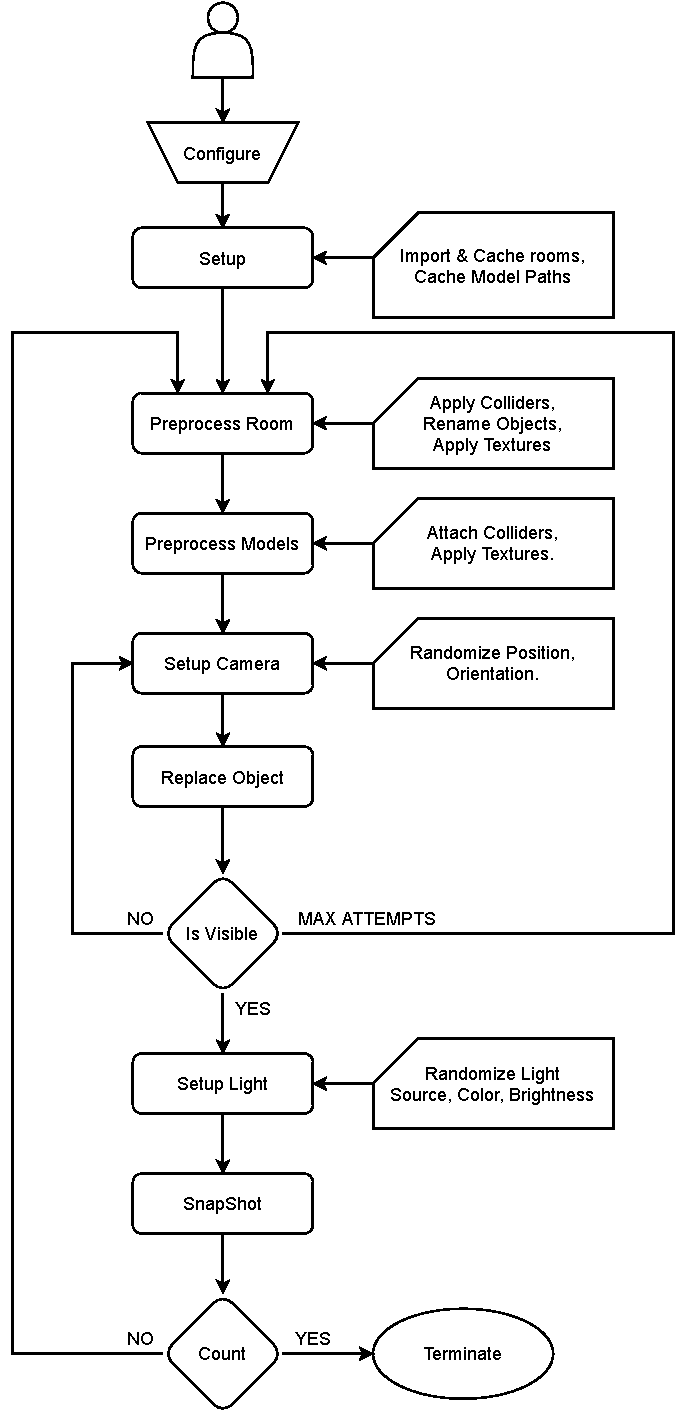
\includegraphics[width=0.9\textwidth, height =1.45\textwidth,valign=m]{/Users/apple/OVGU/Thesis/code/3dReconstruction/report/images/implementation/flowchart}
    \caption{Flowchart for the 3D-Scene Pipeline. The pipeline iterates through the steps till a specified count is reached.}
    \label{fig:flowchart}
\end{figure}

\subsection{Configuration}\label{subsec:configuration}
As an entry point for the user, the application has few parameters which has to be configured.
These need to be inputted by the user using a simple user interface as shown in \autoref{fig:demo1}.
The parameters includes room object path, texture path, model/furniture path and destination path where the images need to saved.
It also includes the categories and total number of required images per category.
The user can also configure camera parameters which include the minimum and macimum distance from the target object and the minimum height of the camera.

\subsection{Modes of operations}\label{subsec:modes-of-operations}
The creation of a dataset can either be automated or by manual intervention.
Automated images may not give us the perfect images that we expect.
There can be some bad lighting, unexpected intersections with other objects, unforeseen camera angles, etc.
To facilitate ease of use for the user, the application has three key pipelines.
After configuring the parameters to create an ersatz environment using Unity,
the user can select any of this pipeline to get automatic snapshots or manual snaps for the models.

The different modes of operation are as follows:
\begin{enumerate}
    \item Single Room pipeline
    \item Manual Room pipeline
    \item Multi Objects pipeline
\end{enumerate}

The single Room pipeline is used to create the dataset with objects in the center of an empty room.
A path to the room can either be provided or else the application imports a default room.
Manual Room pipeline randomizes a furnished room and then replaces the category under observation.
The selection of objects to be replaced is also random.
In this mode, the user has control over taking the snap of the scene.
The user can randomize model and room textures, randomize camera position or manually set it and randomize the lighting conditions.
Once the user is satisfied with the view of the scene, he can save the images with a click of the Snap button.
In Multi Objects pipeline, all the process mentioned in the Manual Room pipeline is automated.
The user will not have control over any of the processes while the program snaps images at random.
Another version of the pipeline which is similar to the Single Room pipeline is the Multi-threaded Single Room pipeline.
As the name suggests, multiple rooms are created based on the number of categories, and for each room, the Single Room pipeline is applied in parallel.
This is an attempt to let the tool perform faster with multi-threading.
The multi-process uses Coroutines which is still a sequential operation, and hence this pipeline needs some work.
To our estimate, even the Multi-threaded pipeline runs 1.5 times faster than Single room pipeline.

\subsection{Setup Rooms and Models}\label{subsec:implementation_setup_rooms_models}
As discussed in \autoref{subsec:scenes-from-scenenet}, we utilize the room objects provided by SceneNet.
For Single Room pipeline, a default empty room prefab is imported, while scenes from SceneNet are imported for Manual and Multi-Object pipelines.
The rooms are in .obj format which each furnitures independent of the room and hence can be modified by the application.
For smooth transition, all the rooms from the given path is loaded as a pre-step into a cache variable.
This process can be time consuming initially, but since it is cached the change of room takes lesser time.
For loading of 3D object like room into the Unity environment at runtime we use the asset `Runtime OBJ Importer'\footnote{https://assetstore.unity.com/packages/tools/modeling/runtime-obj-importer-49547} from Unity asset store.
This library helps to import both the object meshes and the material into any Unity environment.

\subsection{Preprocess Rooms and Models}\label{subsec:implementation_preprocess_rooms_models}
In preprocessing step, the rooms and models are assigned properties required in the further steps.
Each object in the room is attached with a collider component, which as the name suggests detects collisions.
This component is needed to detect a object either using raycast or when it actually intersects with the target object.
We utilize \emph{MeshCollider} component for the same.

We then rename all the objects in the room to some common names used in day-to-day life.
Example: cushions, pillows, lamp, laptop, etc.
Though the objects in scenes from SceneNet are named with some common objects, the name contains unintelligible texts appended with it.
Hence, we rename them to pre-defined list of common object.
If any object does not belong in the list, it will be renamed as `misc'.
Some edge cases where more than one name resemble the same object are also handled.
For example: TV and Television are both renamed to TV.

Similarly, the models from Pix3D are also preprocessed.
Each model is attached with a MeshCollider, in this case to detect collision with the other objects in the scene.
In case of target models, we can even apply gravity so that it appears on the floor.
However, we chose to place it using its dimensions, which also makes it appear to be on the floor.

Then we apply textures for both room and models as described in \autoref{subsec:implementation_randomised-texture}.

\subsection{Randomized Texture}\label{subsec:implementation_randomised-texture}
We randomly allocate textures to each object, ensuring that each category has the same texture to make the scene more uniform.
The objects in the scene are renamed to standard objects seen in day-to-day life.
The textures are grouped together to these names as folder names.
A dictionary is created for all the gameobjects, such that we keep track of all the unique categories.
Each category is assigned a single texture using \emph{Texture2D.LoadImage}.

Another randomized entity is the skybox.
Skybox acts as the outdoor scene for a given room.
For each of the pipelines, skybox changes for every snap taken.
Samples for changing skyboxes is as shown in \autoref{fig:skybox samples}.

\subsection{Setup Camera}\label{subsec:implementation_camera}
As a device through which the users can visualize the ersatz environment we utilize Unity's default Camera object.
We use a single camera whose coordinates or transforms can be changed at runtime.
Few of the camera parameters like height of the camera, minimum and maximum distance from the target object, can be decided by the user in the initial configuration.
A CameraHelper class, which has both the main camera and the target object as its parameter then selects a random point in the space with these constraints for the camera to be placed.
The camera is then rotated towards the target object using the `Transform.LookAt' API.
The next step is the check if the target object is still within the frame.
This is achieved by casting a ray from the camera using \emph{Physics.Linecast}, which tells us if the ray is intersecting a collider object.
To make the frame realistic, we avoid unrelatable views by applying a constraint on the camera position and make sure that the camera is in front of the target object within an angle of 60 degrees.

\subsection{Replacing target Objects}\label{subsec:implementation_replacing-target-objects}
Once the room is set up using SceneNet~\cite{McCormac2017}, which contains objects from ShapeNet~\cite{shapenet2015}, the objects are renamed such that it matches the classes for the Pix3D dataset.
Since a given scene can have more than one category under observation, a single model is chosen randomly out of all the present models.
The chosen model is replaced with a model in Pix3D of the same category, by making it invisible using \emph{GameObject.SetActive}.
In case the replaced model is intersecting with any other models in the scene, we make it invisible.
After the snapshot is taken, the scene is reset to the original, and the next model is imported.


\subsection{Setup Lighting}\label{subsec:implementation_lighting}

Unity has a wide variety of lighting system.
We utilize three types of lights offered in Unity.

\begin{itemize}
    \item Point light
    \item Spotlight
    \item Directional light
\end{itemize}

Point lights act as indoor lights for the room, the range of which can be varied.
We pre-define six light patterns for a room with a cuboid shape.
Knowing the bounds of the room, we decide how to place the lights by randomly select 1 to 6 lights with corresponding light patterns on the ceiling.
For the spotlight, only a single light is placed a meter above the target object.
This light gives a variation that focuses only on the target object.
Both point and spot-light have color variation along with varying brightness.
Directional light is the default light settings in Unity.
For our environment this acts a natural Sun Light.
This is specifically effective when the room has windows forming more realistic shadows.
In this case, we modulate the brightness, and the angle at which the rays are emitted, which simulates different times of the day.
Additional to these different types of light, we give ceilings the property of light with limited brightness as we observed that the entire room does not light up for a single light source.
This is similar to what BlenderProc~\cite{dlr139317} do for all scenarios.
Samples of different lighting conditions and shadows with varying colors are displayed in \autoref{fig:Lighting and shadows}.


\subsection{Snapshots with ML-ImageSynthesis}\label{subsec:snapshots-with-ml-imagesynthesis}

ML-ImageSynthesis~\footnote{https://bitbucket.org/Unity-Technologies/ml-imagesynthesis} is a library provided by Unity to support synthetic dataset creation.
It supports the following G-buffers Image segmentation, Object categorization, Optical flow, Depth, Normals, etc.
G-buffers is basically a collective term to represent light properties that are aggregated to give the final rendering.
In image segmentation, each object is assigned a unique color.
In object categorization, each category of the objects is assigned a single color.
For optical flow, each pixel is colored depending on Unity's per-pixel Motion Vectors with respect to the camera.
The depth map is, as the word suggests, the distance of each pixel from the camera encoded in 8-bit channels of the PNG image.
Normals are color encoding based on the orientation of the object with respect to the camera.
For the snapshot, each of these properties is assigned a hidden camera and has each one overrides rendering scene with custom shaders to generate corresponding output.
These camera outputs can be seen in editor mode by changing the display window.
Samples of G-buffer collected for the dataset are as shown in \autoref{fig:G-buffers-samples}.

\begin{figure}
    \centering
        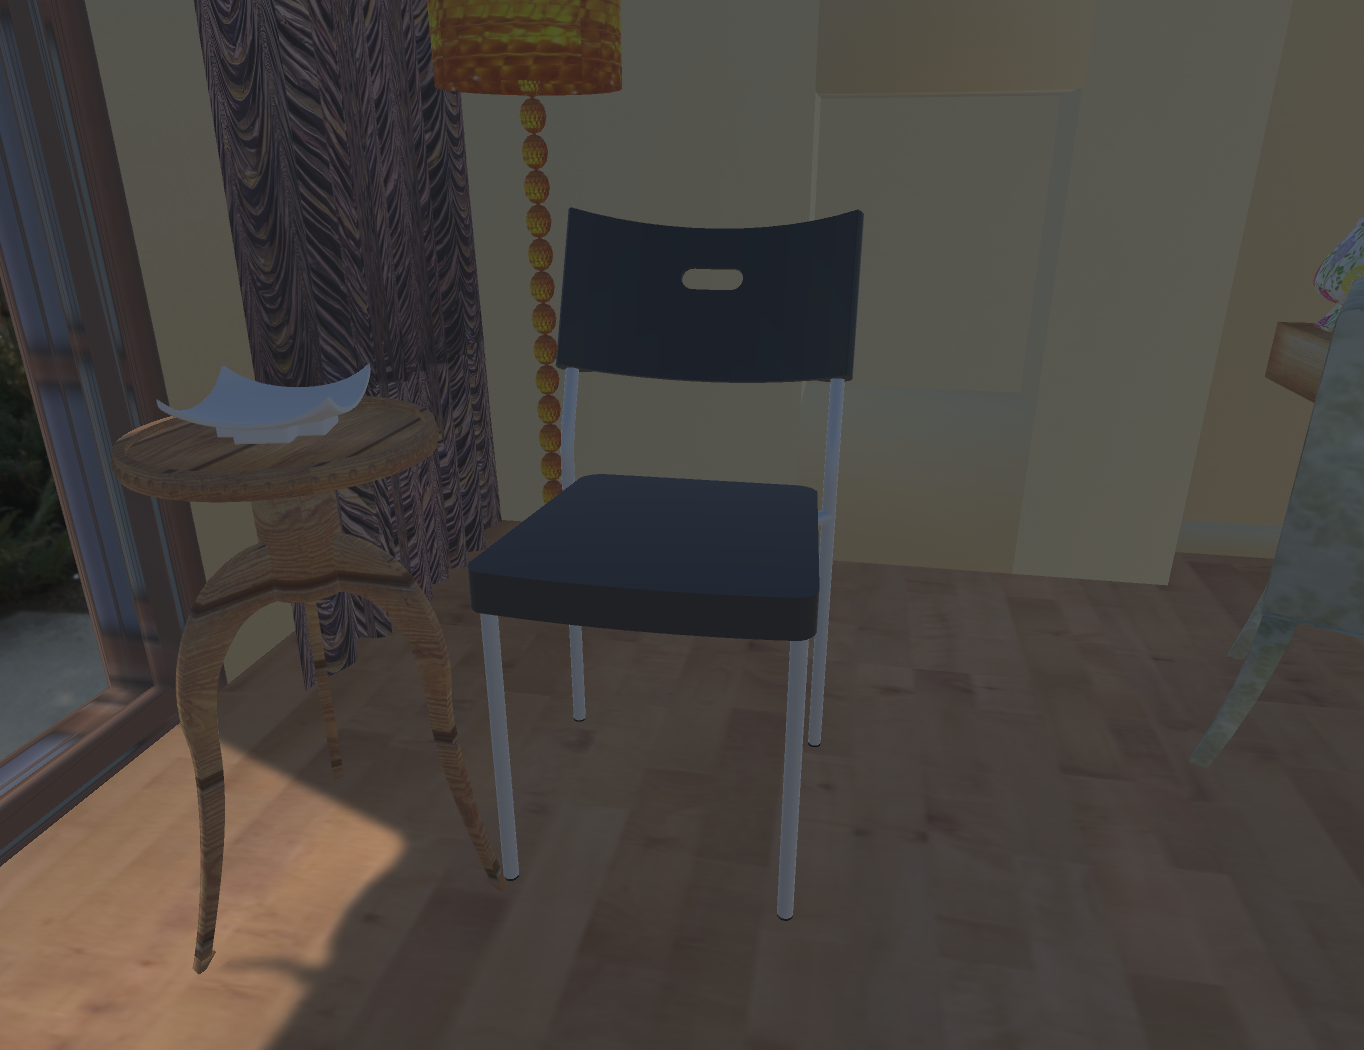
\includegraphics[width=.19\linewidth]{/Users/apple/OVGU/Thesis/code/3dReconstruction/report/images/implementation/gbuffers/0_img}
        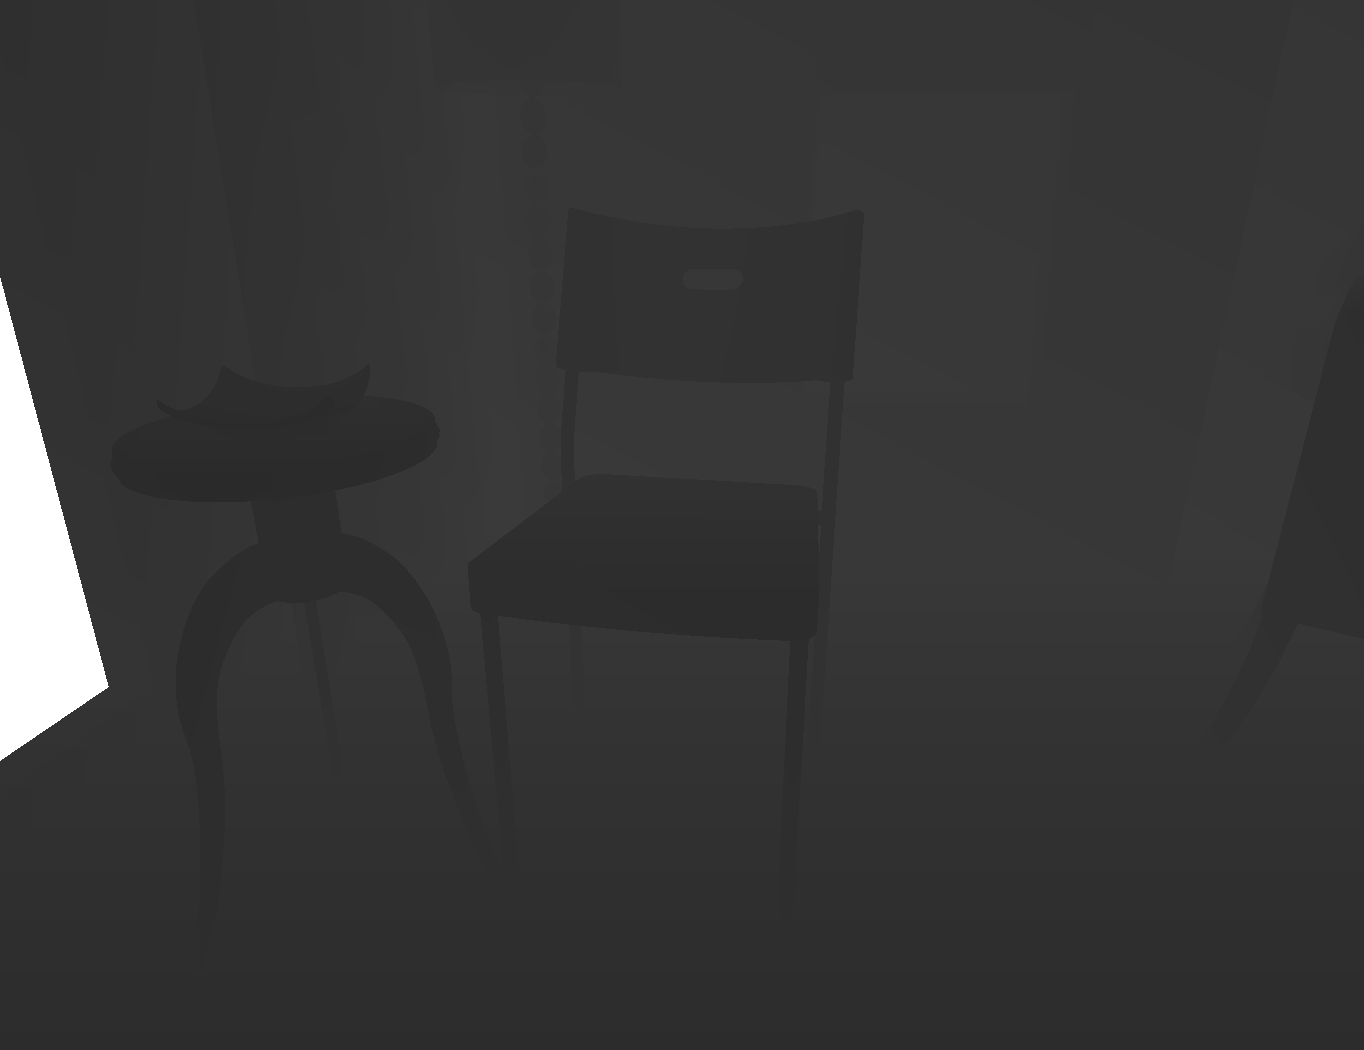
\includegraphics[width=.19\linewidth]{/Users/apple/OVGU/Thesis/code/3dReconstruction/report/images/implementation/gbuffers/0_depth}
        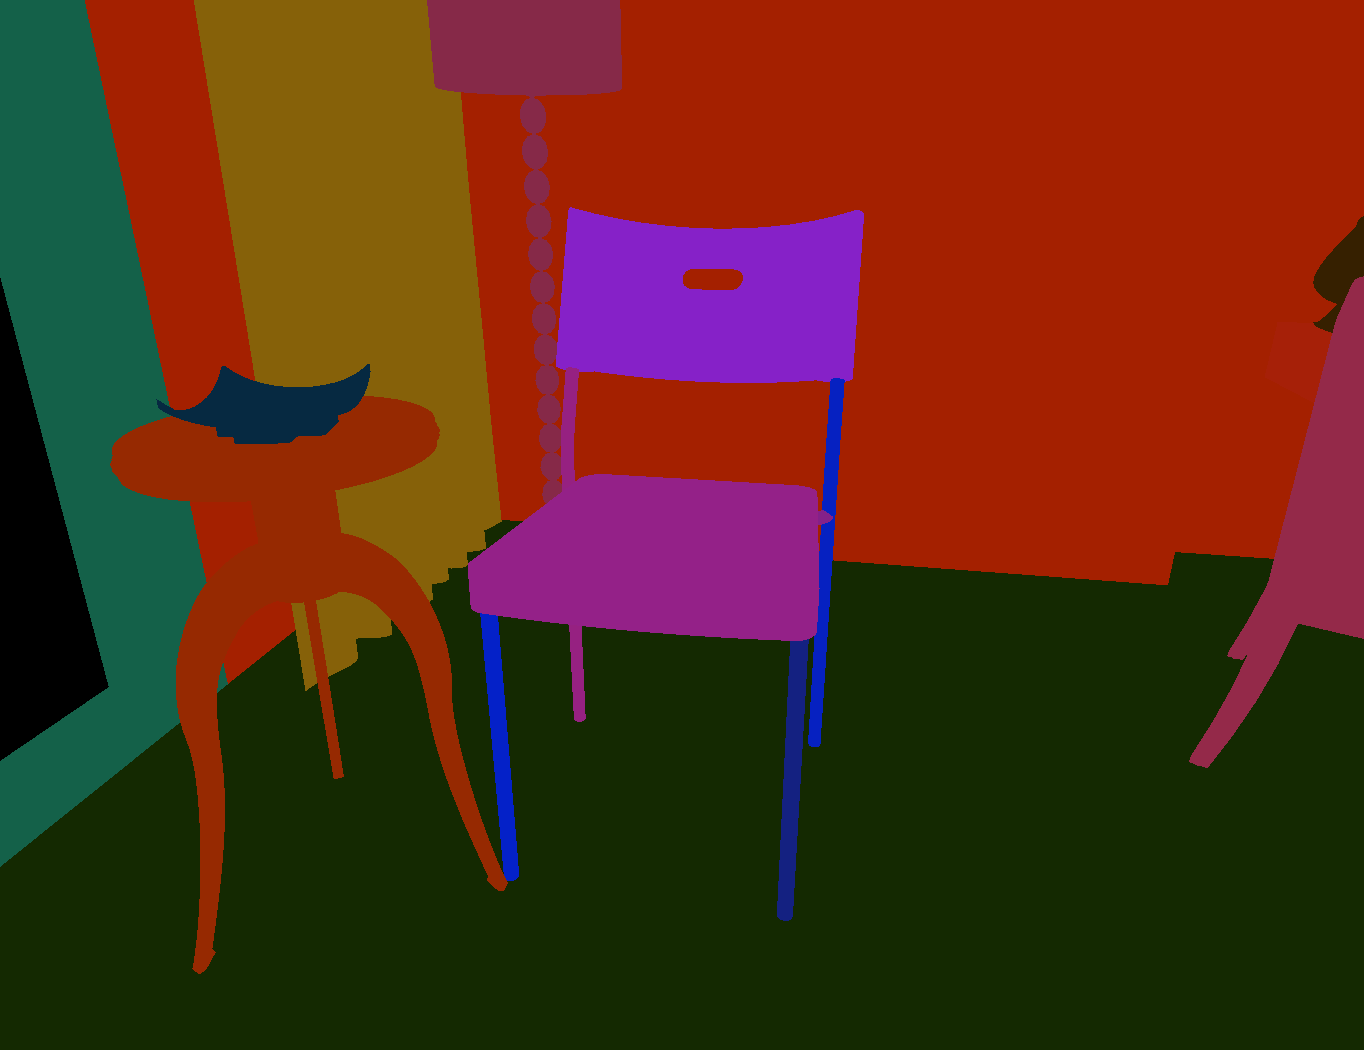
\includegraphics[width=.19\linewidth]{/Users/apple/OVGU/Thesis/code/3dReconstruction/report/images/implementation/gbuffers/0_id}
        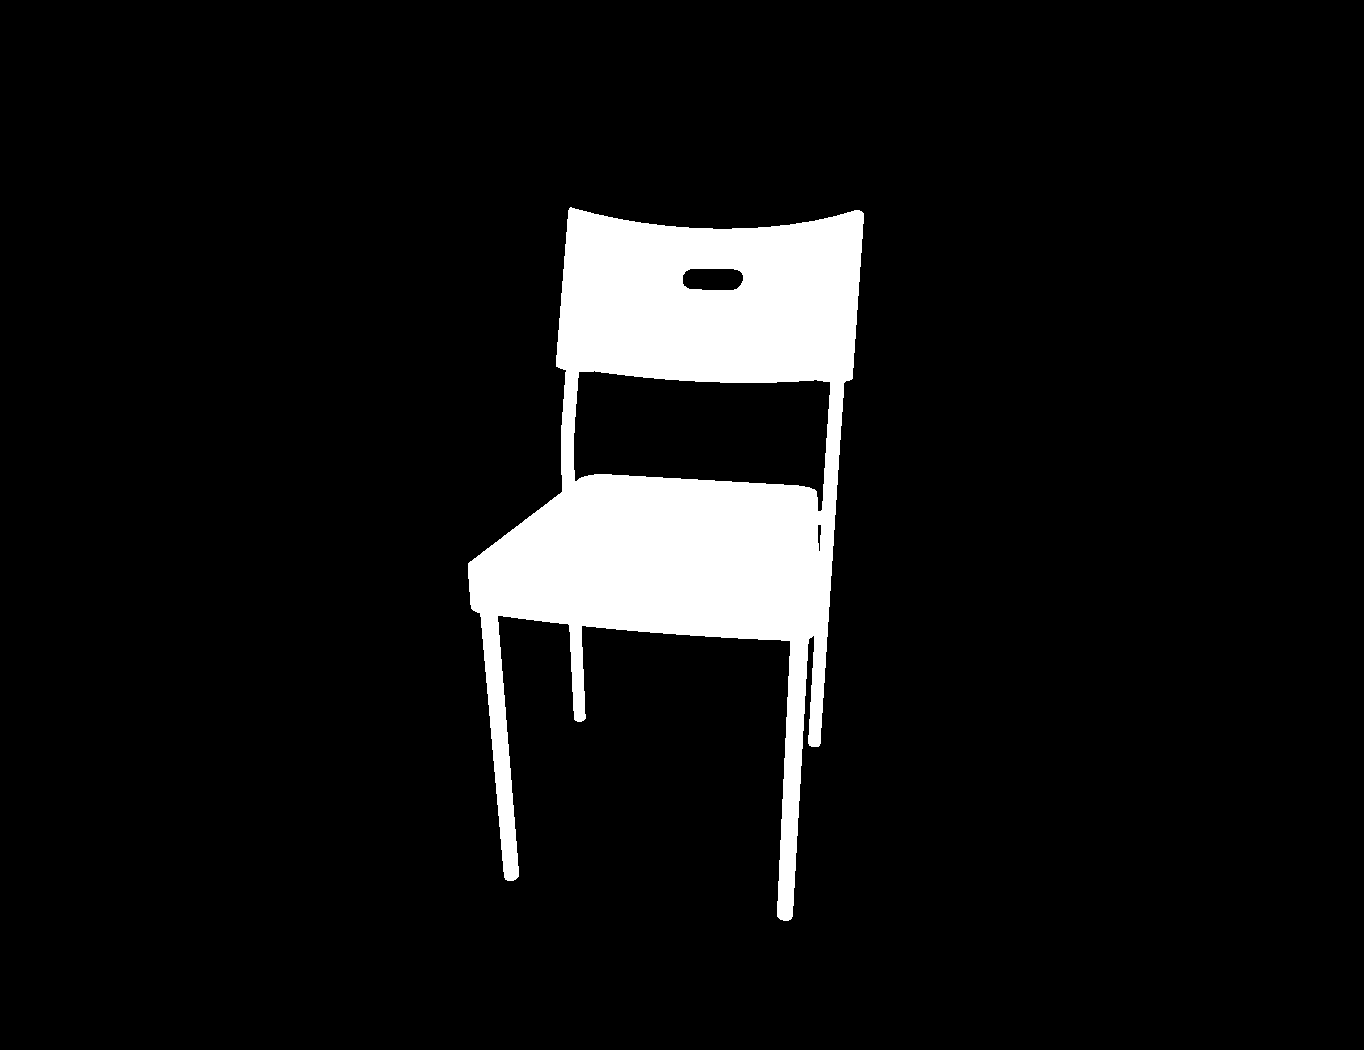
\includegraphics[width=.19\linewidth]{/Users/apple/OVGU/Thesis/code/3dReconstruction/report/images/implementation/gbuffers/0_layer}
        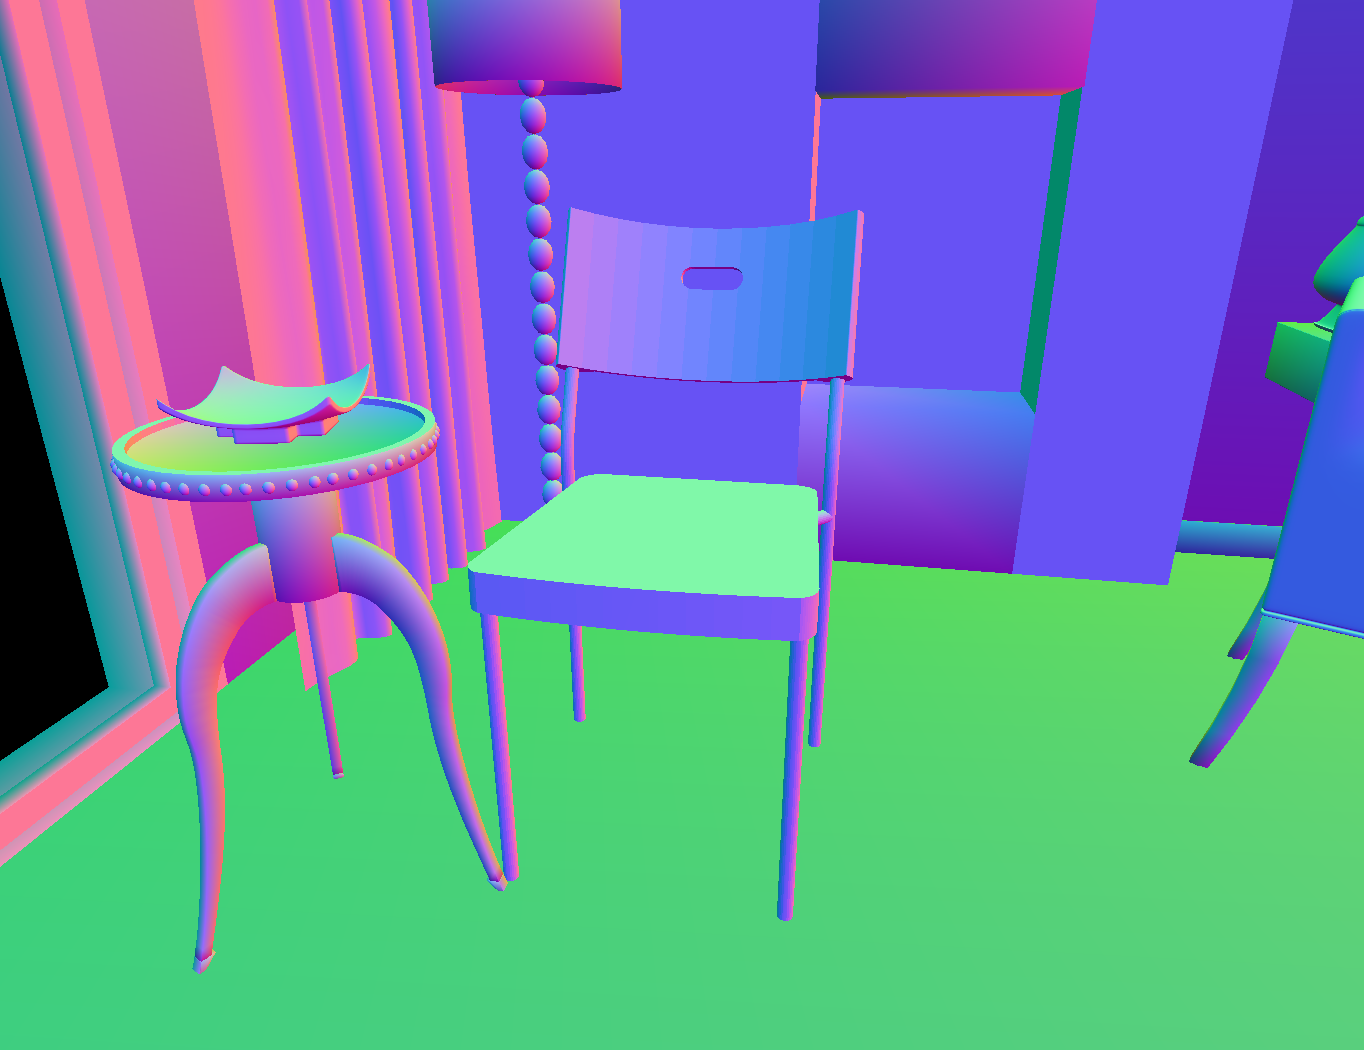
\includegraphics[width=.19\linewidth]{/Users/apple/OVGU/Thesis/code/3dReconstruction/report/images/implementation/gbuffers/0_normals}\\
        \vspace{0.1cm}
        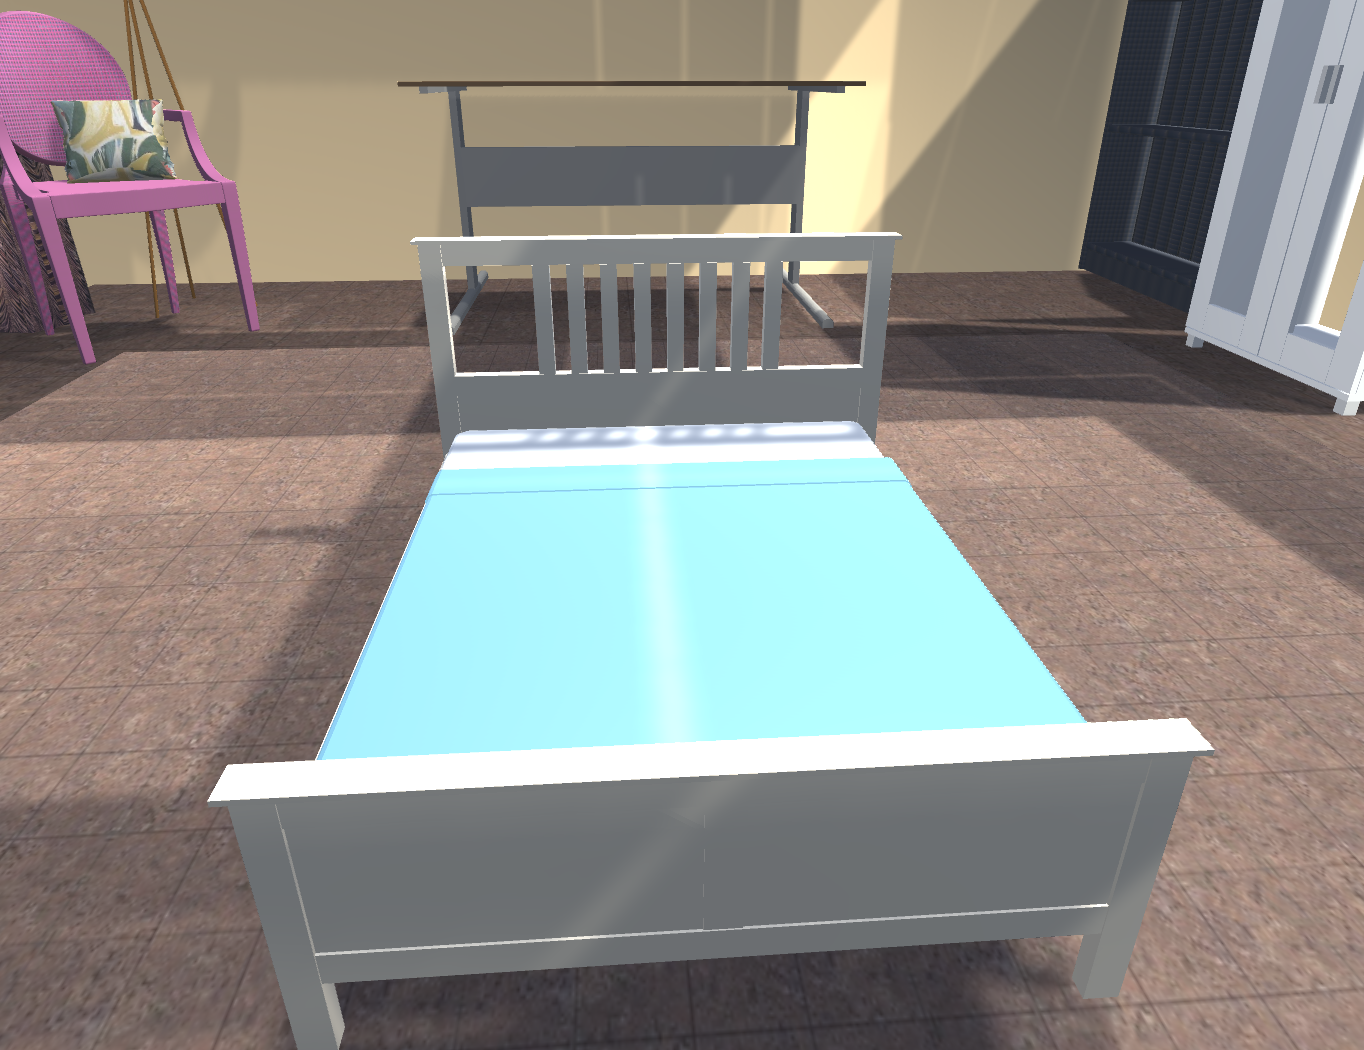
\includegraphics[width=.19\linewidth]{/Users/apple/OVGU/Thesis/code/3dReconstruction/report/images/implementation/gbuffers/1_img}
        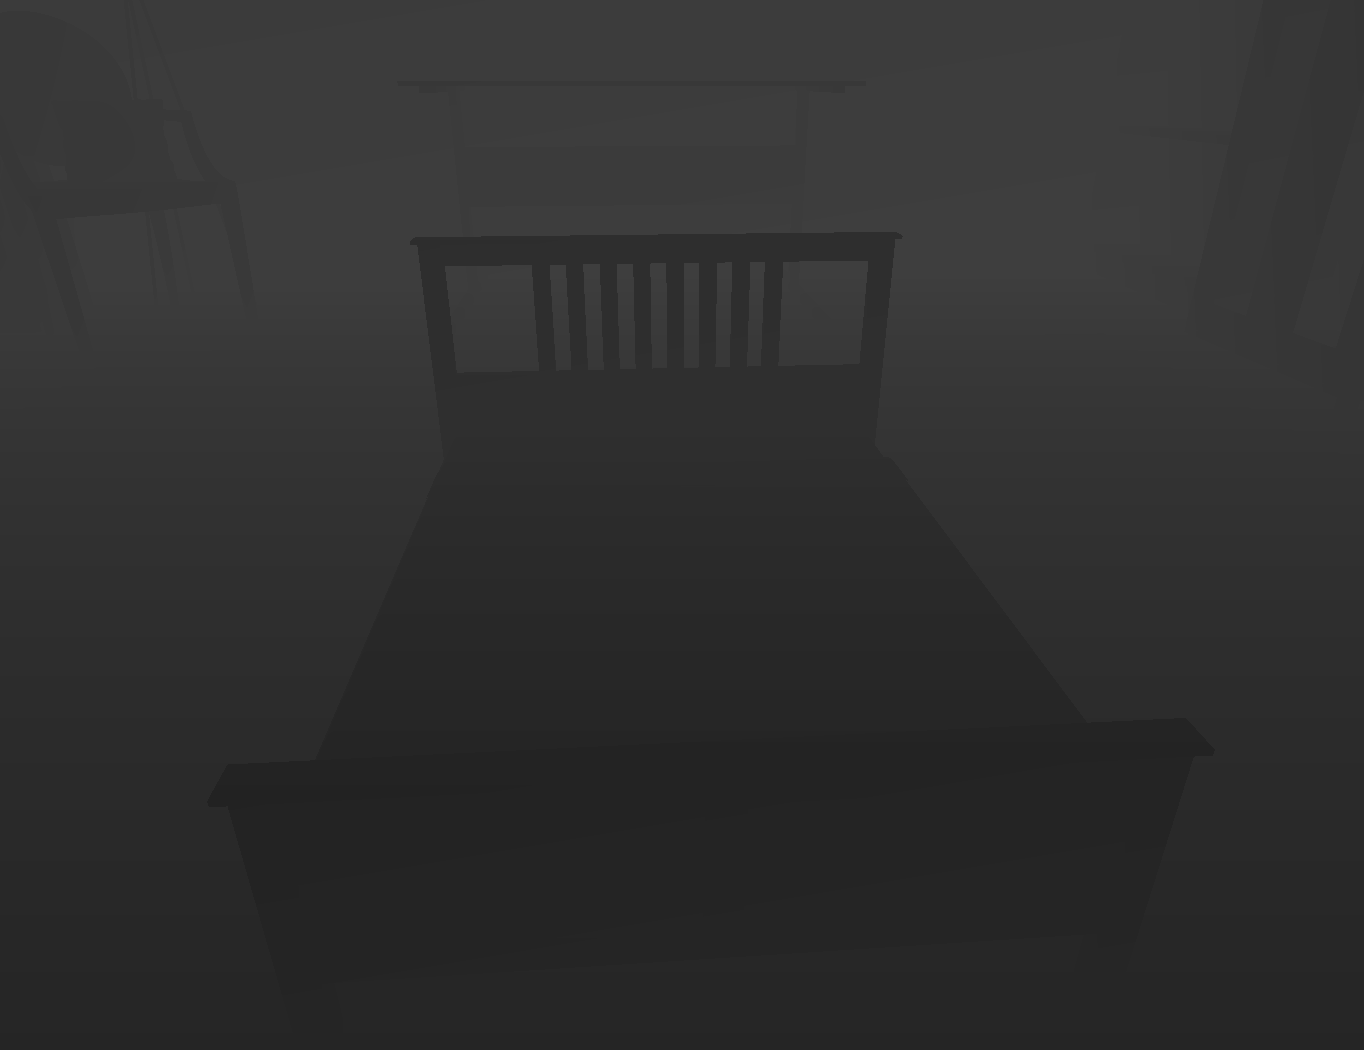
\includegraphics[width=.19\linewidth]{/Users/apple/OVGU/Thesis/code/3dReconstruction/report/images/implementation/gbuffers/1_depth}
        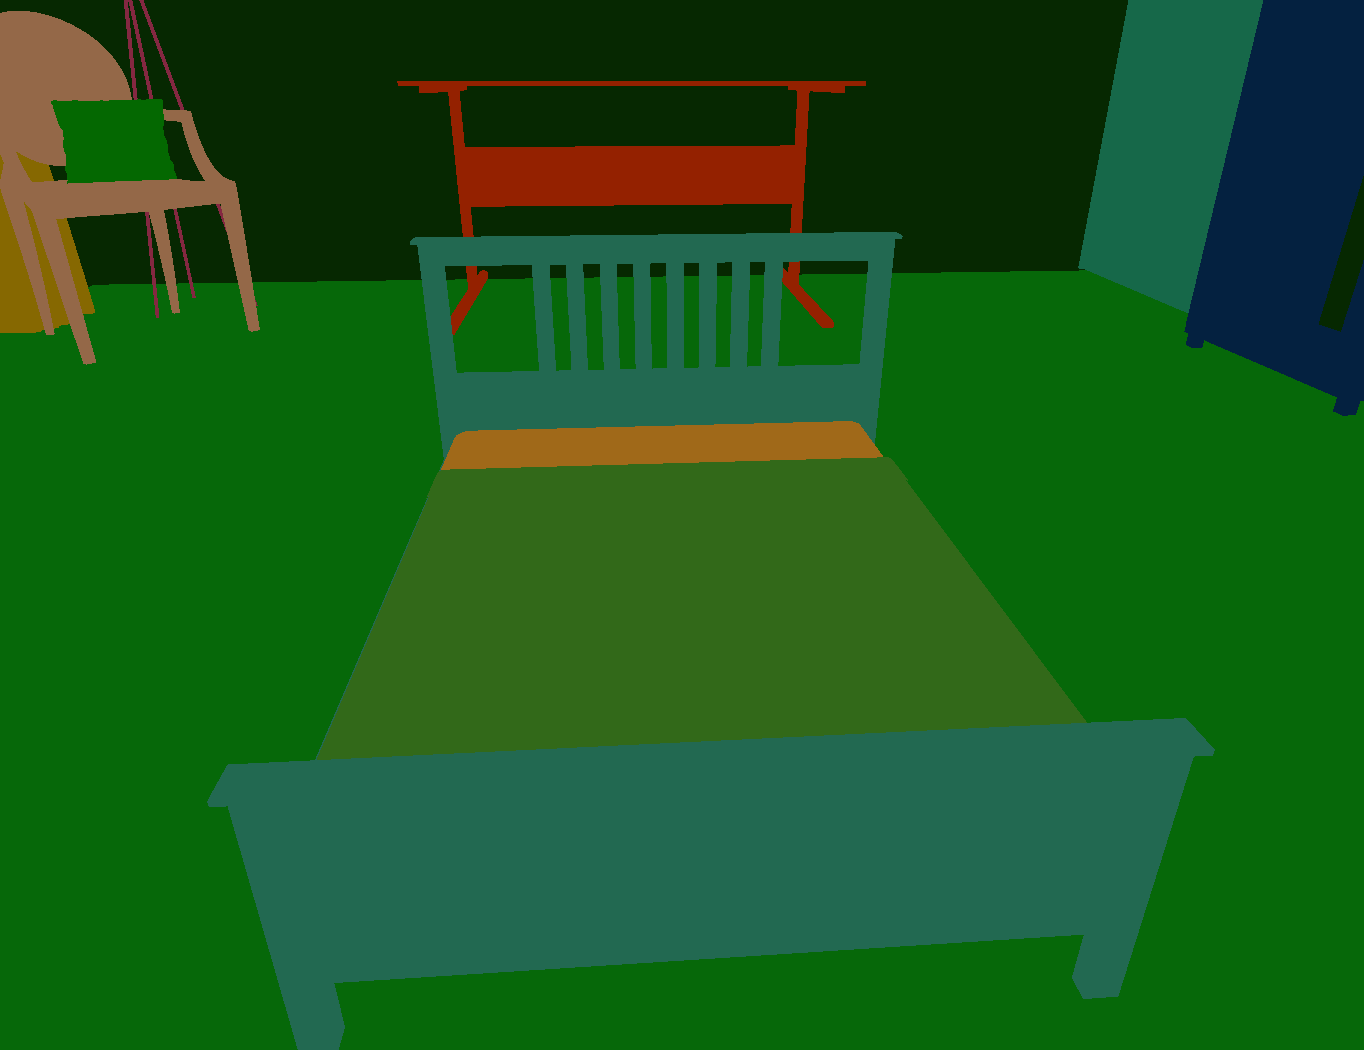
\includegraphics[width=.19\linewidth]{/Users/apple/OVGU/Thesis/code/3dReconstruction/report/images/implementation/gbuffers/1_id}
        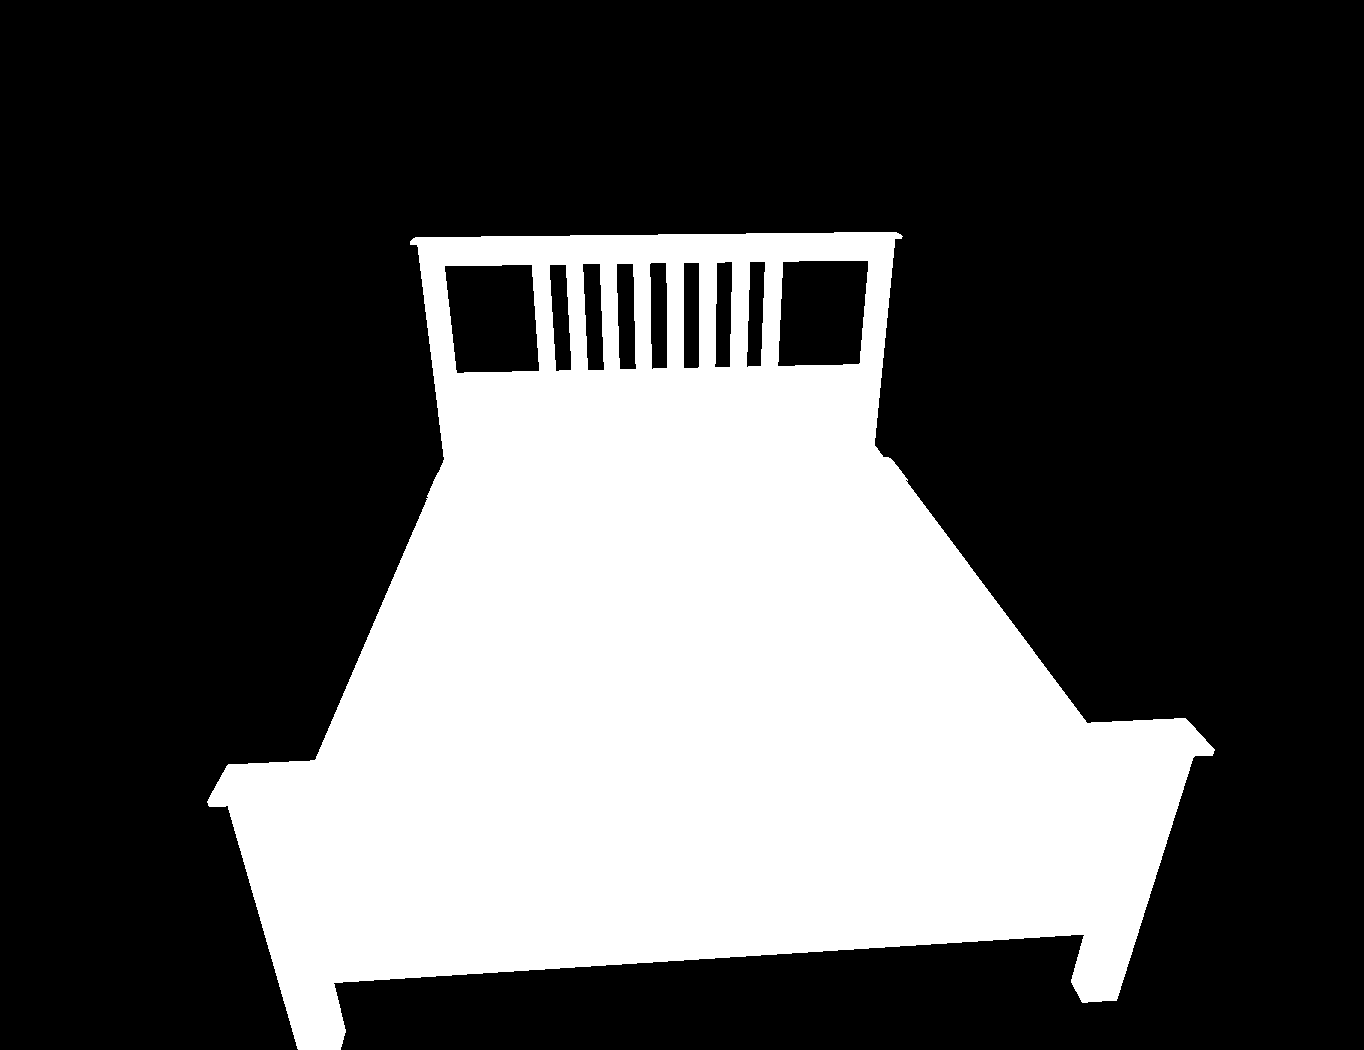
\includegraphics[width=.19\linewidth]{/Users/apple/OVGU/Thesis/code/3dReconstruction/report/images/implementation/gbuffers/1_layer}
        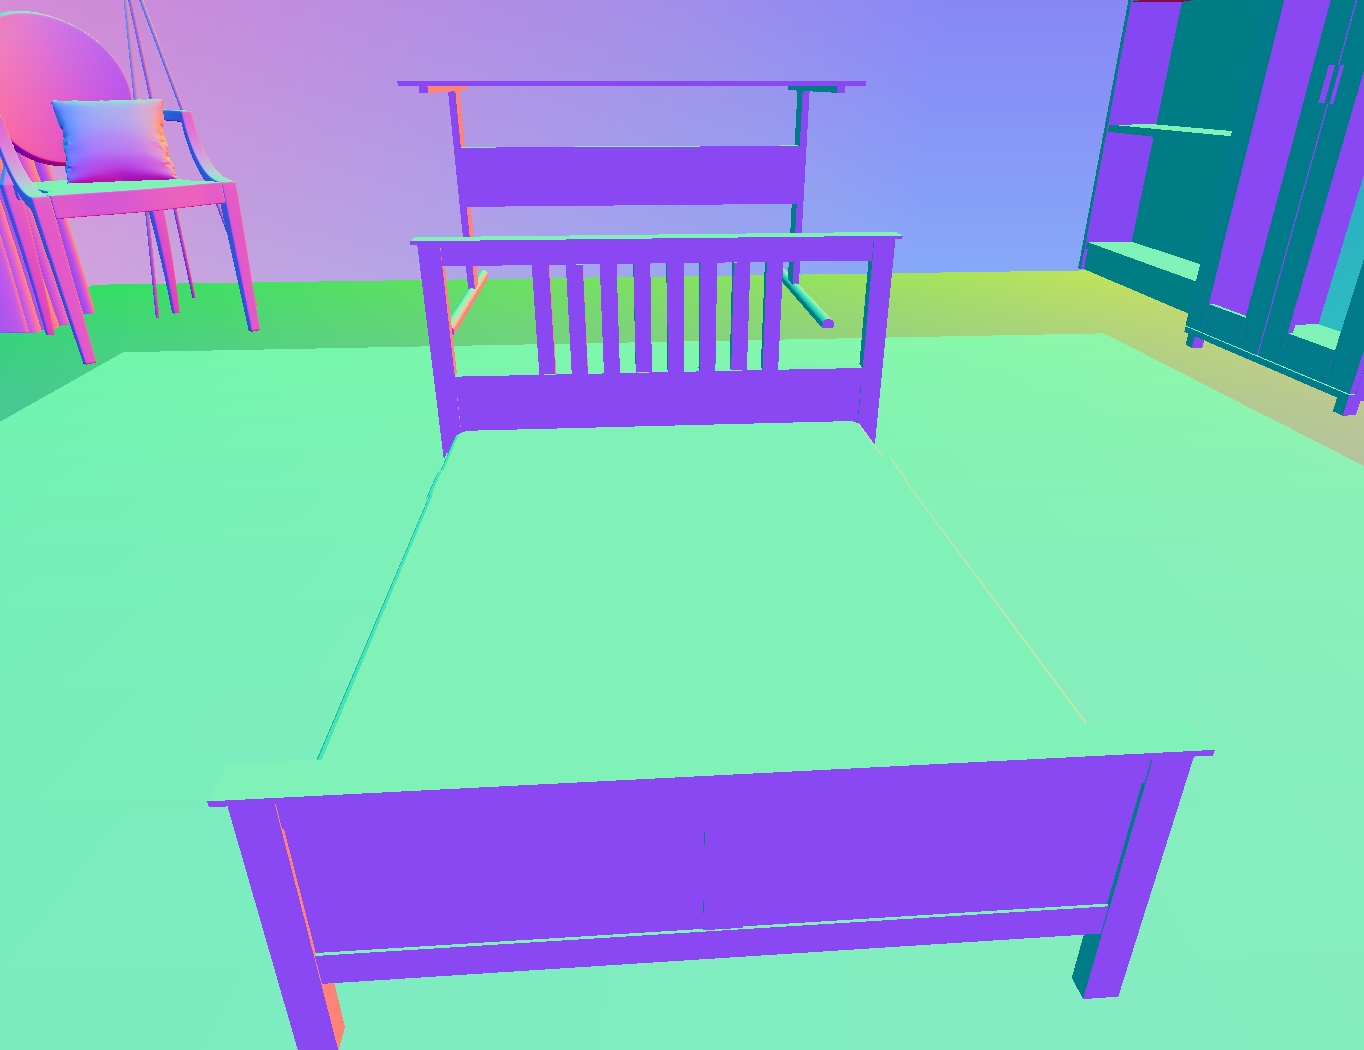
\includegraphics[width=.19\linewidth]{/Users/apple/OVGU/Thesis/code/3dReconstruction/report/images/implementation/gbuffers/1_normals}\\
        \vspace{0.1cm}

        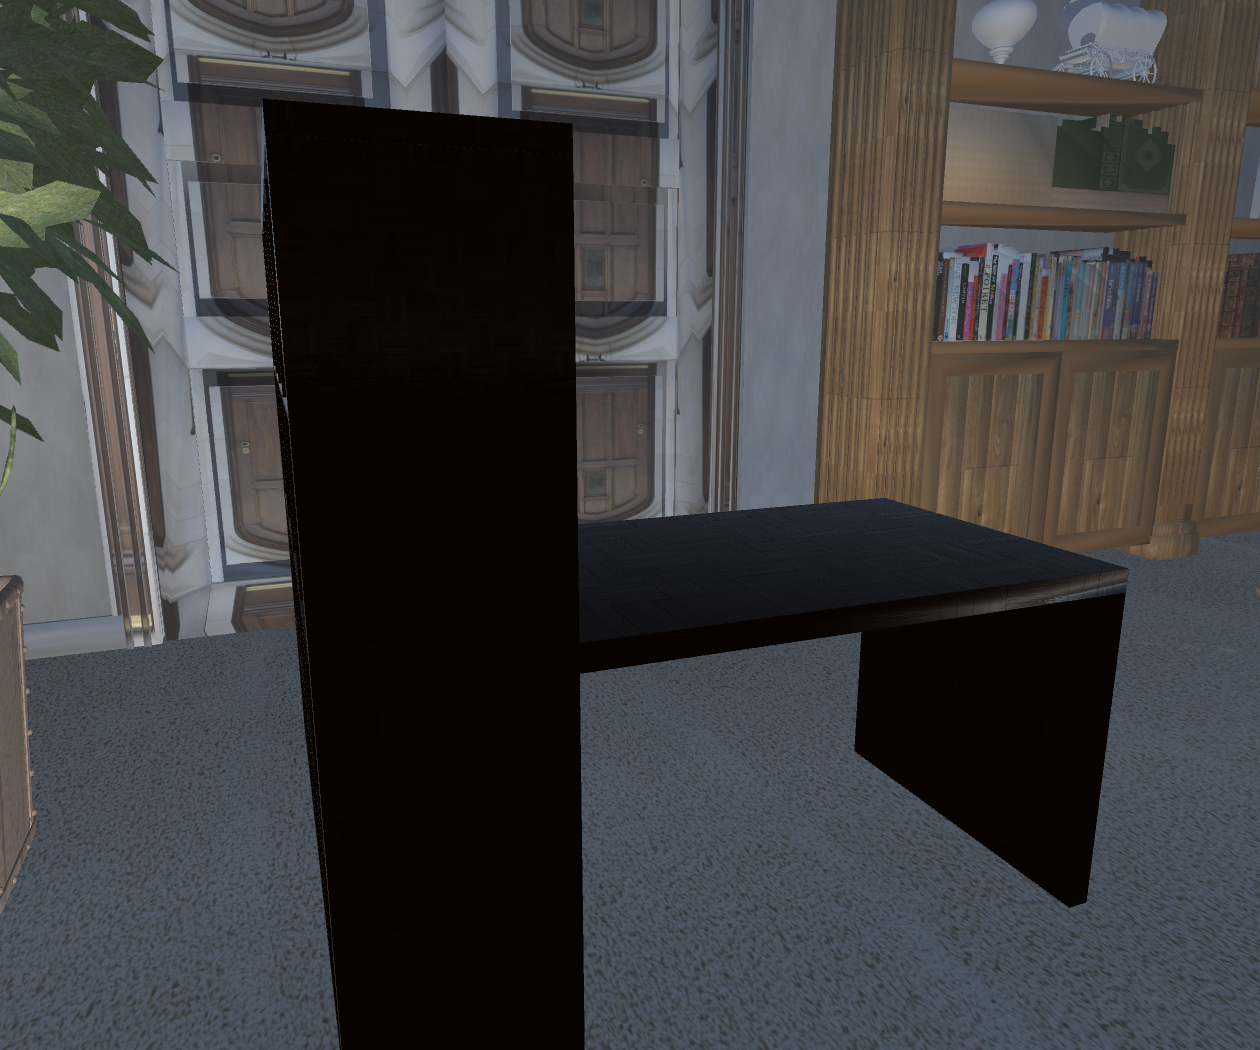
\includegraphics[width=.19\linewidth]{/Users/apple/OVGU/Thesis/code/3dReconstruction/report/images/implementation/gbuffers/2_img}
        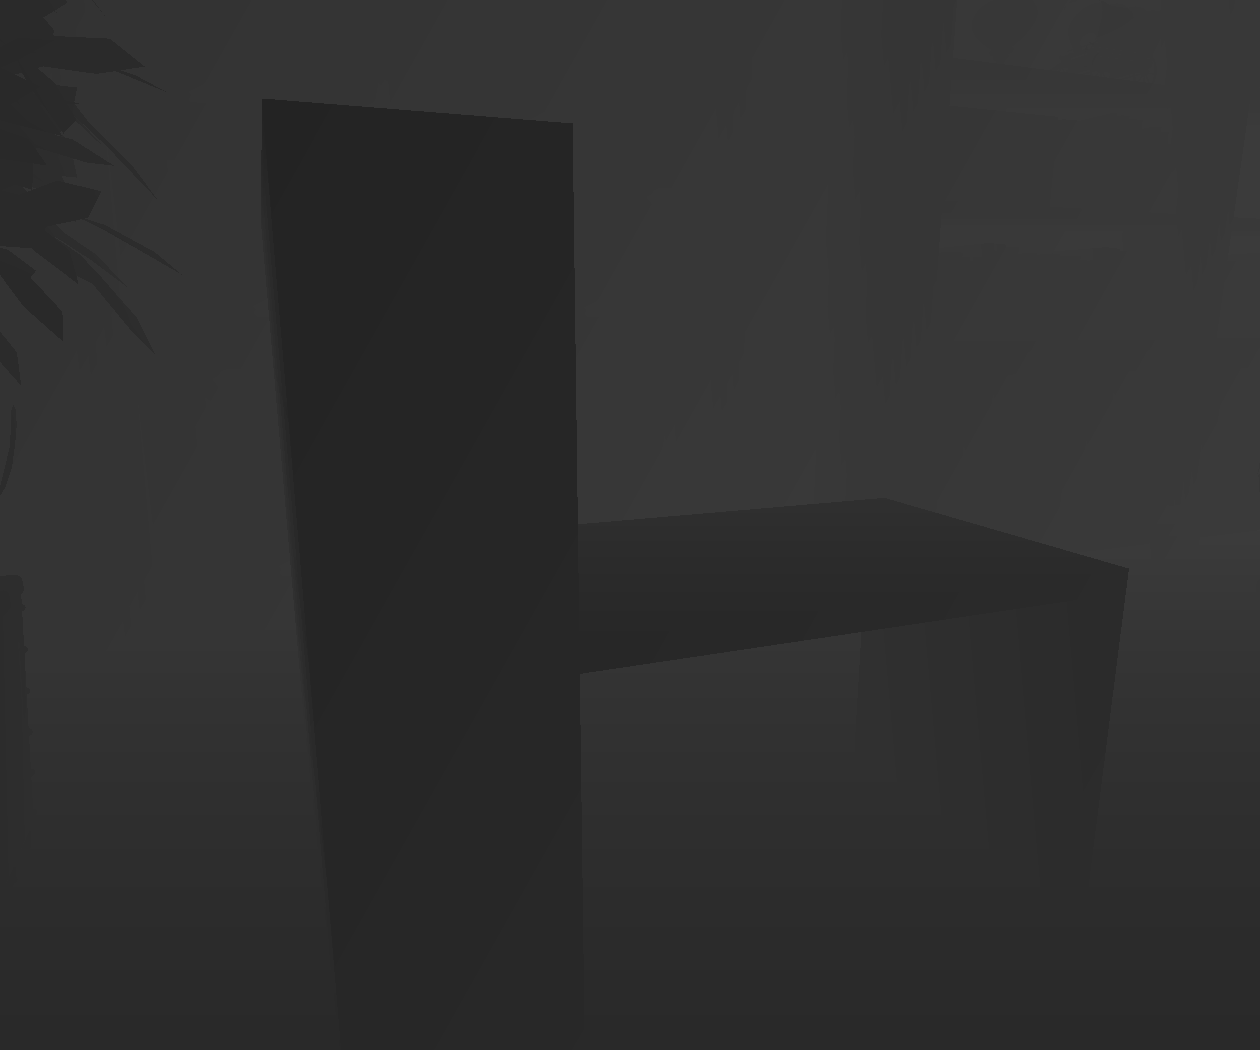
\includegraphics[width=.19\linewidth]{/Users/apple/OVGU/Thesis/code/3dReconstruction/report/images/implementation/gbuffers/2_depth}
        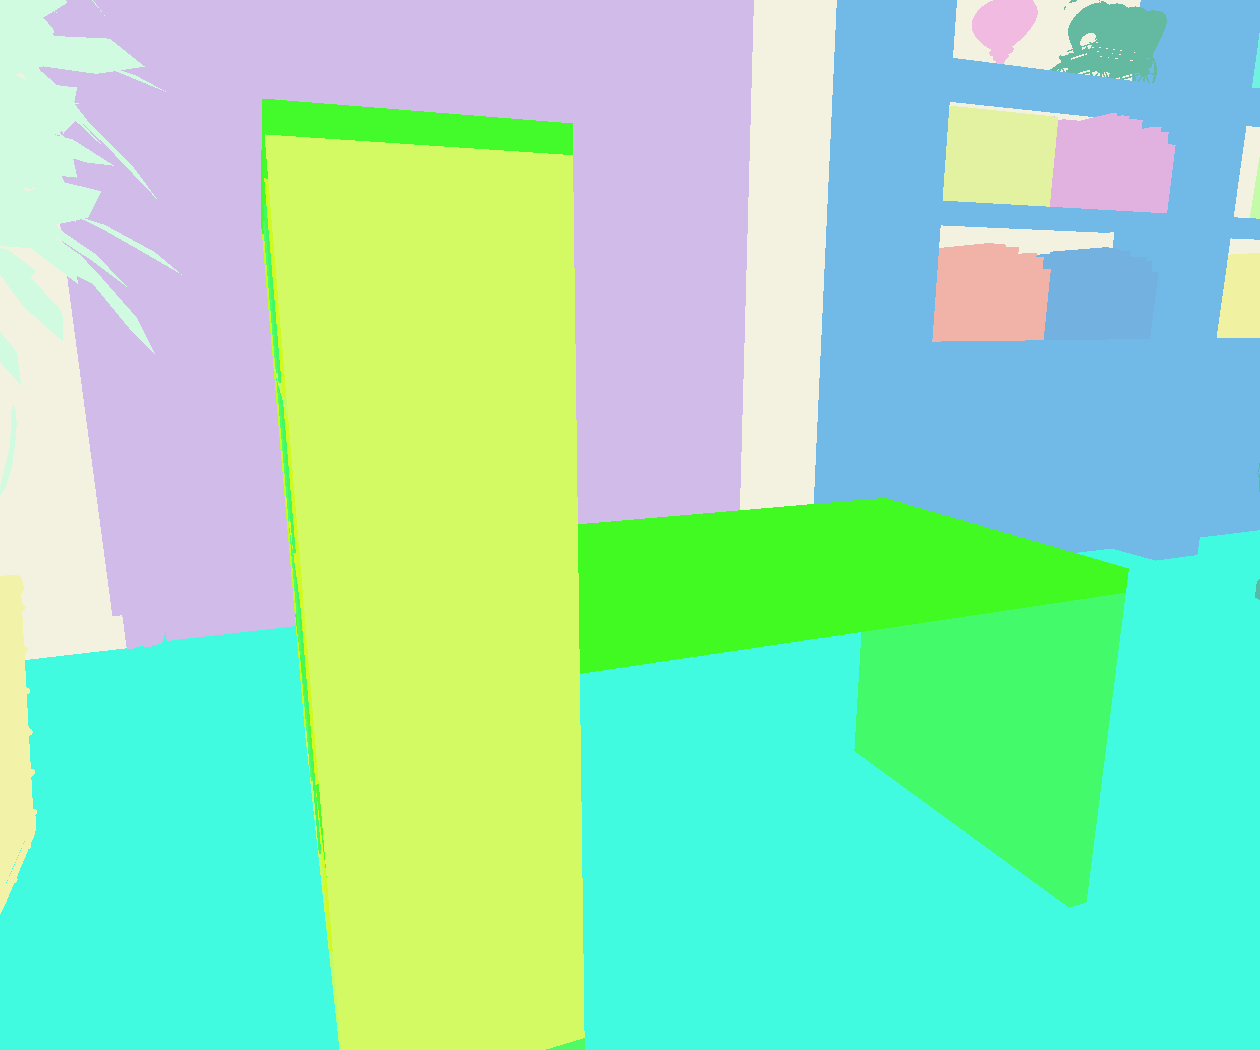
\includegraphics[width=.19\linewidth]{/Users/apple/OVGU/Thesis/code/3dReconstruction/report/images/implementation/gbuffers/2_id}
        
\includegraphics[width=.19\linewidth]{/Users/apple/OVGU/Thesis/code/3dReconstruction/report/images/implementation/gbuffers/2_layer}
        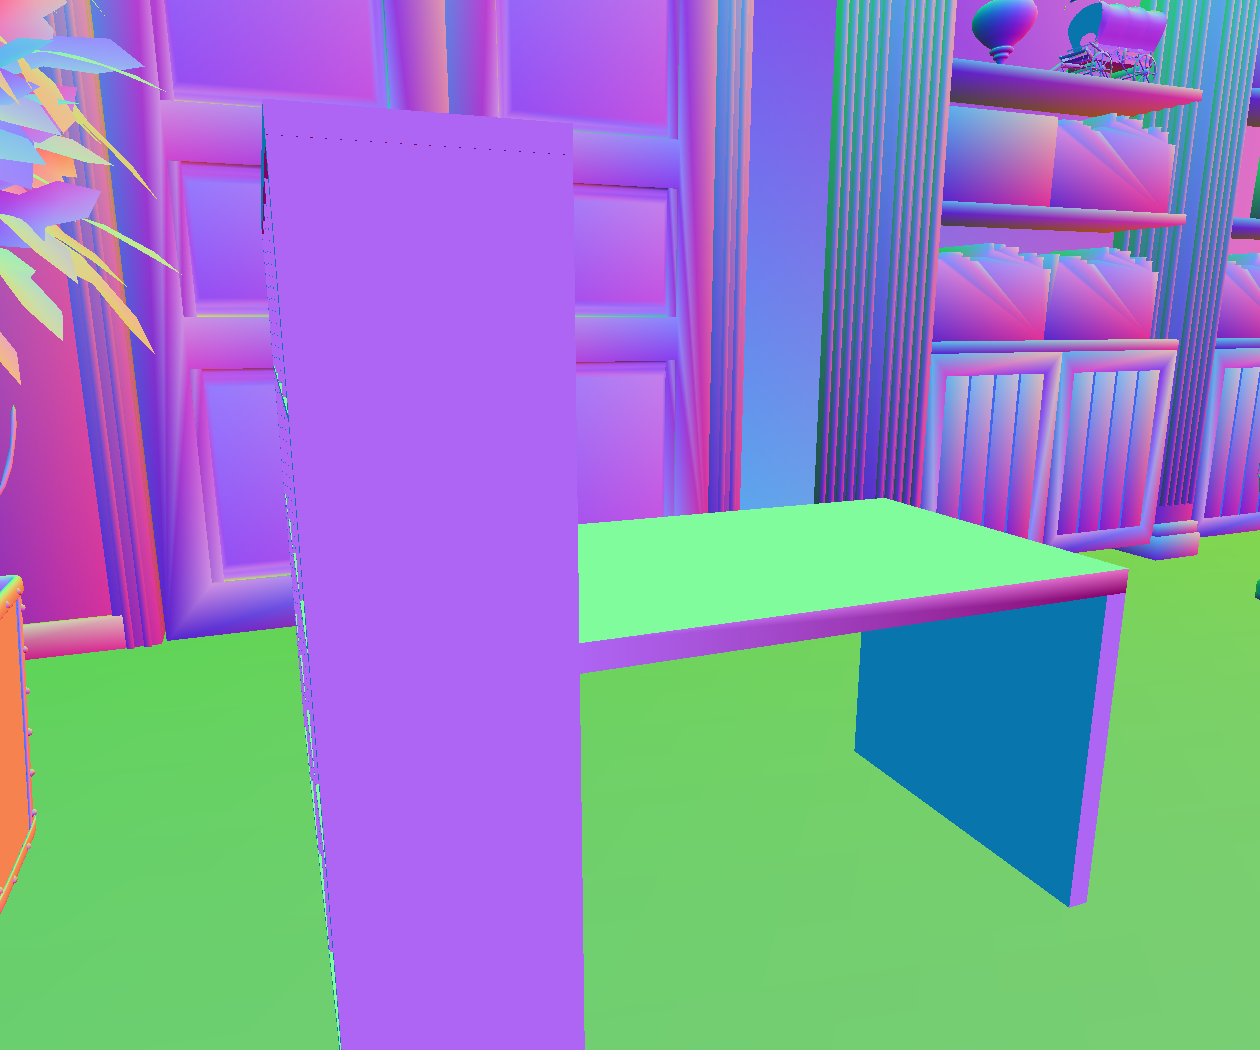
\includegraphics[width=.19\linewidth]{/Users/apple/OVGU/Thesis/code/3dReconstruction/report/images/implementation/gbuffers/2_normals}\\
        \vspace{0.1cm}
        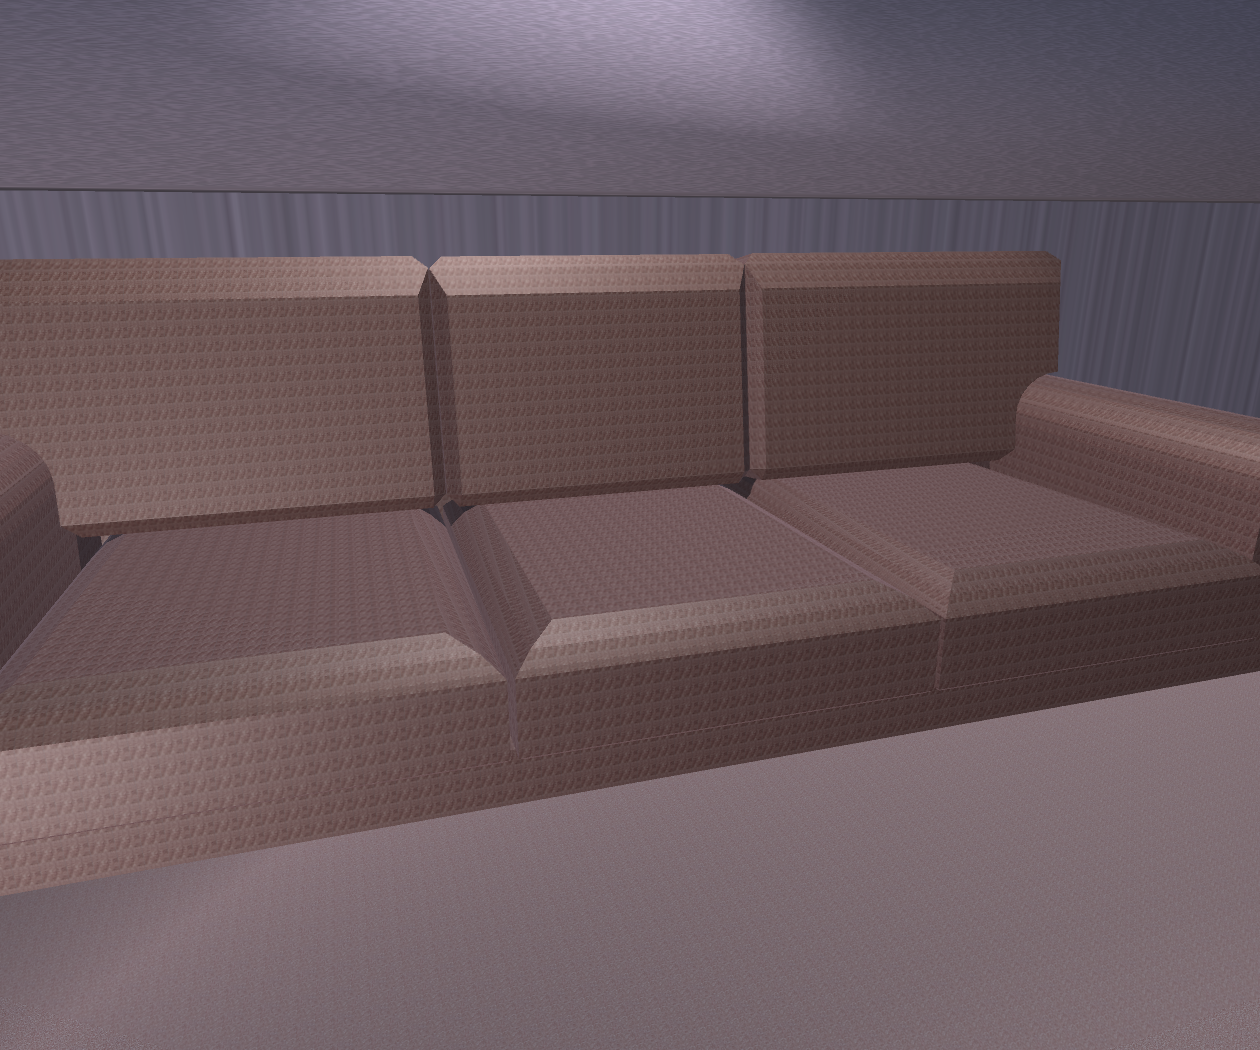
\includegraphics[width=.19\linewidth]{/Users/apple/OVGU/Thesis/code/3dReconstruction/report/images/implementation/gbuffers/3_img}
        
\includegraphics[width=.19\linewidth]{/Users/apple/OVGU/Thesis/code/3dReconstruction/report/images/implementation/gbuffers/3_depth}
        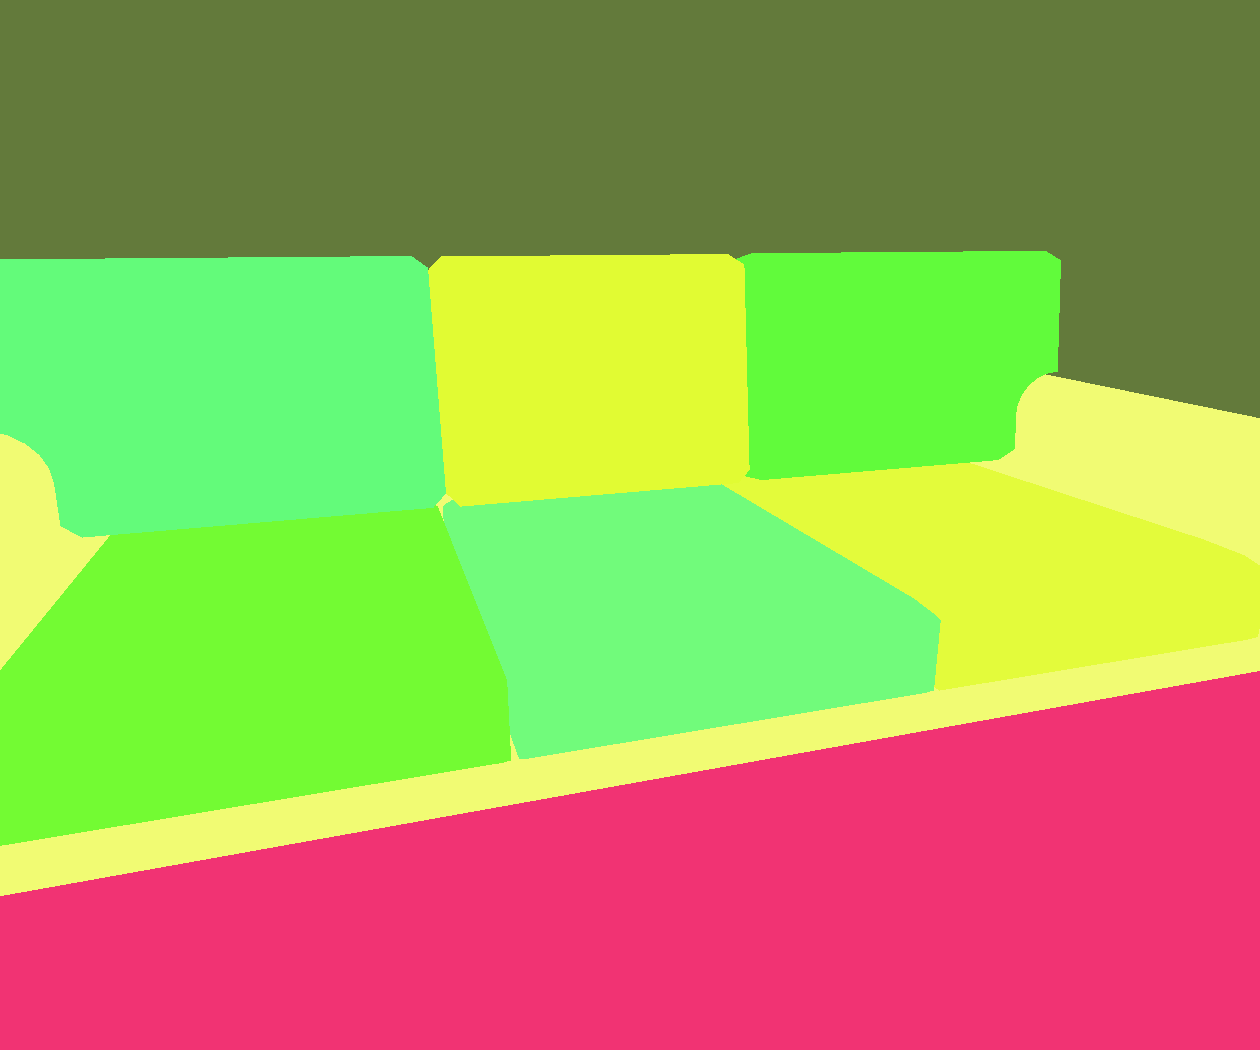
\includegraphics[width=.19\linewidth]{/Users/apple/OVGU/Thesis/code/3dReconstruction/report/images/implementation/gbuffers/3_id}
        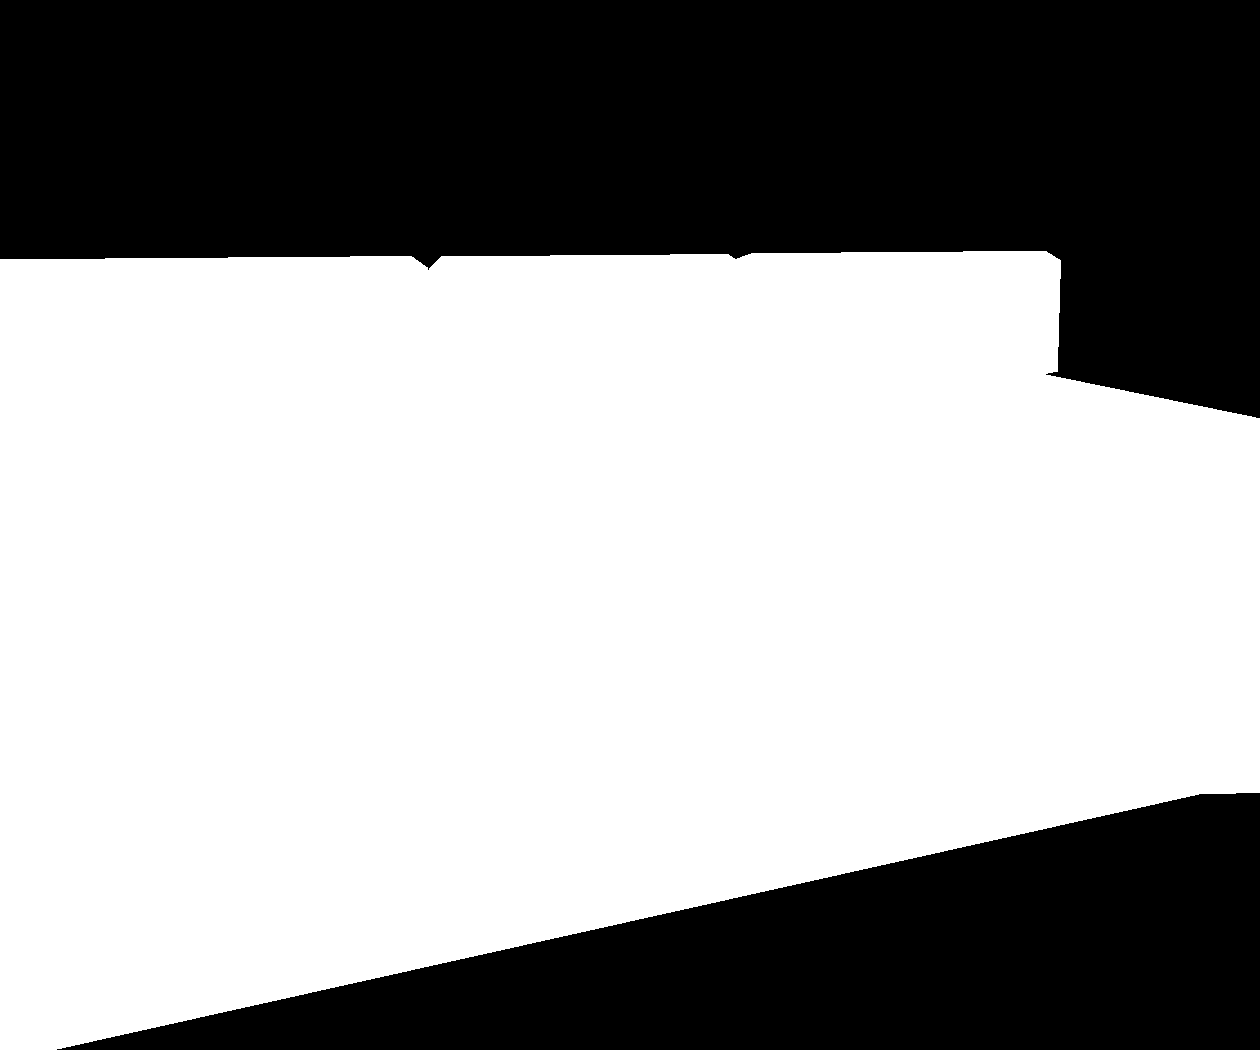
\includegraphics[width=.19\linewidth]{/Users/apple/OVGU/Thesis/code/3dReconstruction/report/images/implementation/gbuffers/3_layer}
        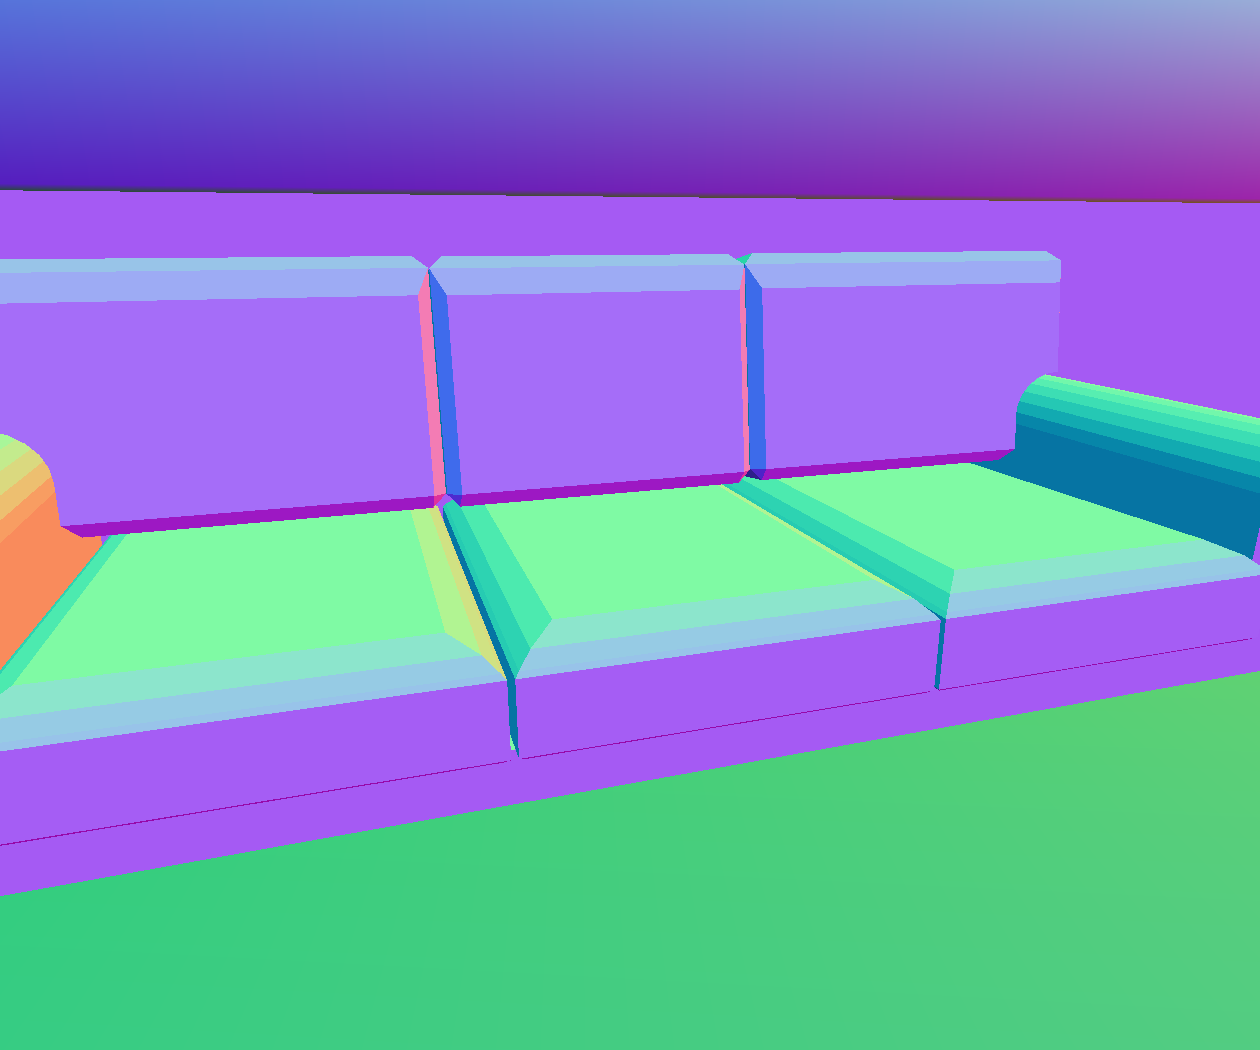
\includegraphics[width=.19\linewidth]{/Users/apple/OVGU/Thesis/code/3dReconstruction/report/images/implementation/gbuffers/3_normals}\\
    \vspace{0.1cm}

        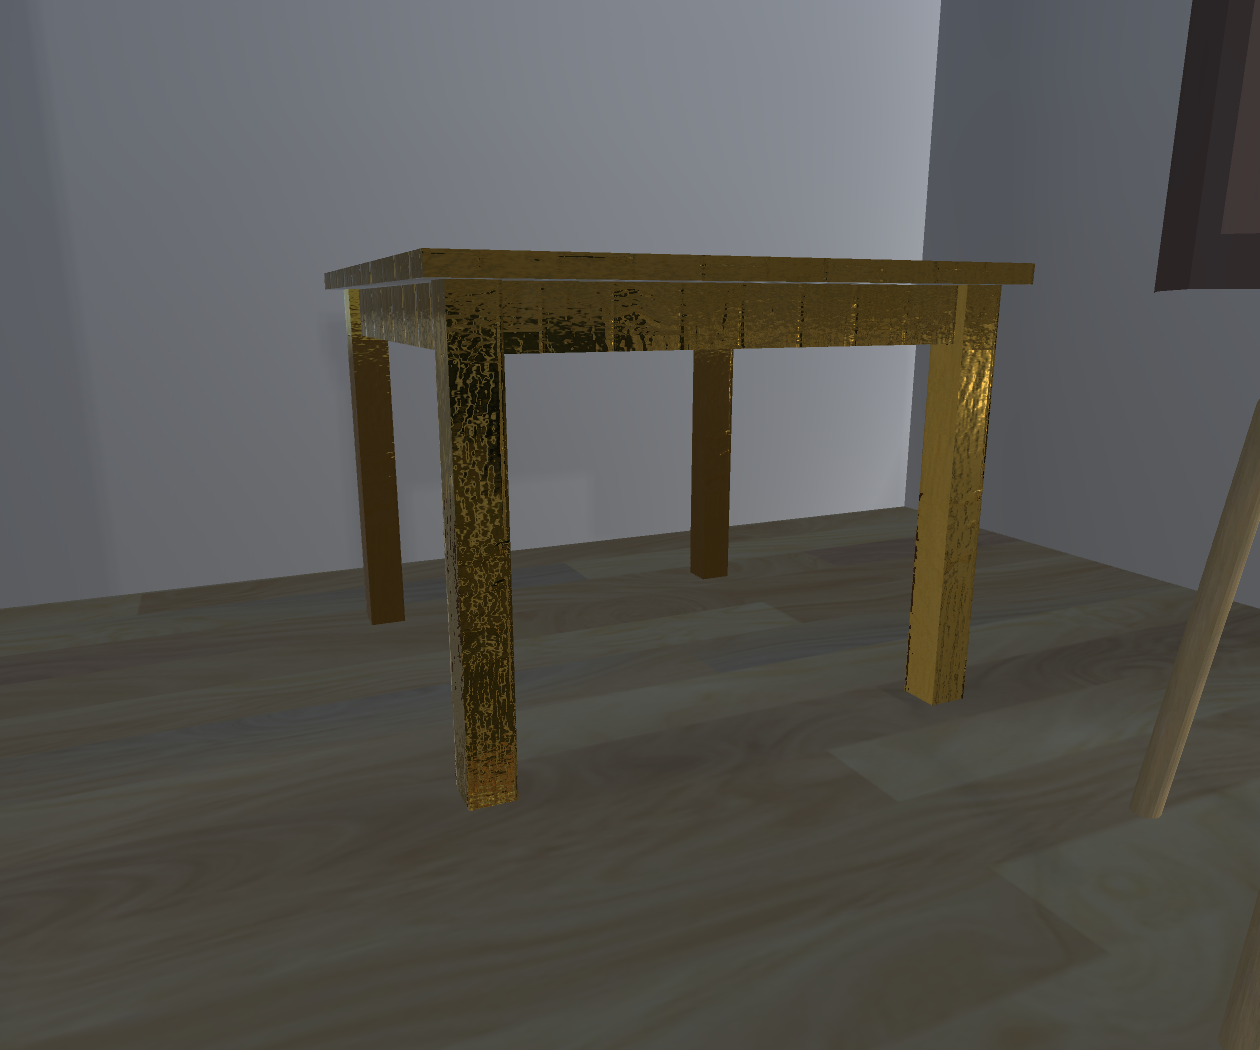
\includegraphics[width=.19\linewidth]{/Users/apple/OVGU/Thesis/code/3dReconstruction/report/images/implementation/gbuffers/4_img}
        
\includegraphics[width=.19\linewidth]{/Users/apple/OVGU/Thesis/code/3dReconstruction/report/images/implementation/gbuffers/4_depth}
        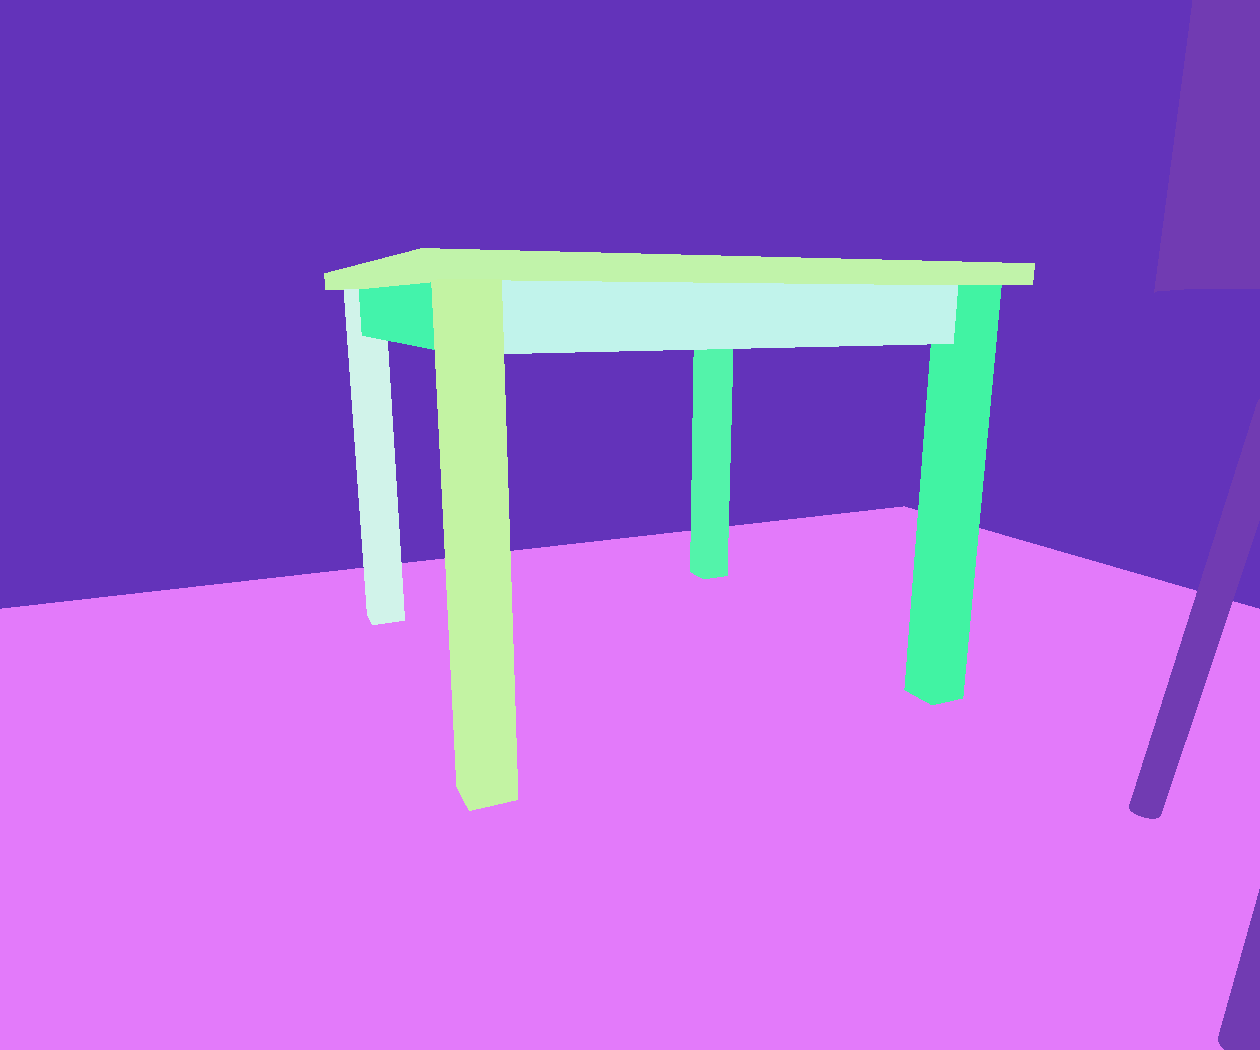
\includegraphics[width=.19\linewidth]{/Users/apple/OVGU/Thesis/code/3dReconstruction/report/images/implementation/gbuffers/4_id}
        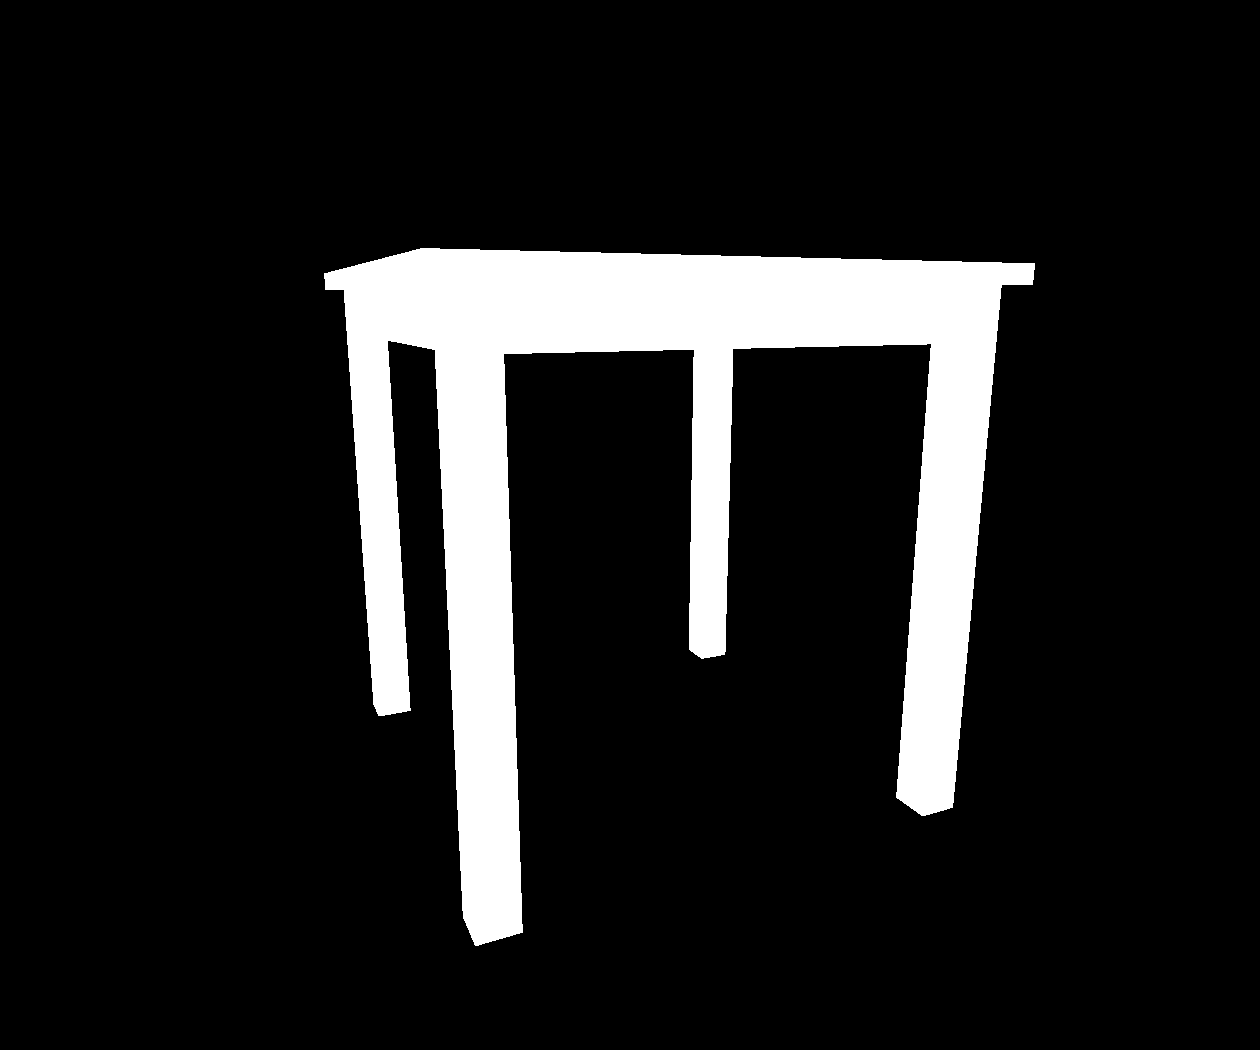
\includegraphics[width=.19\linewidth]{/Users/apple/OVGU/Thesis/code/3dReconstruction/report/images/implementation/gbuffers/4_layer}
        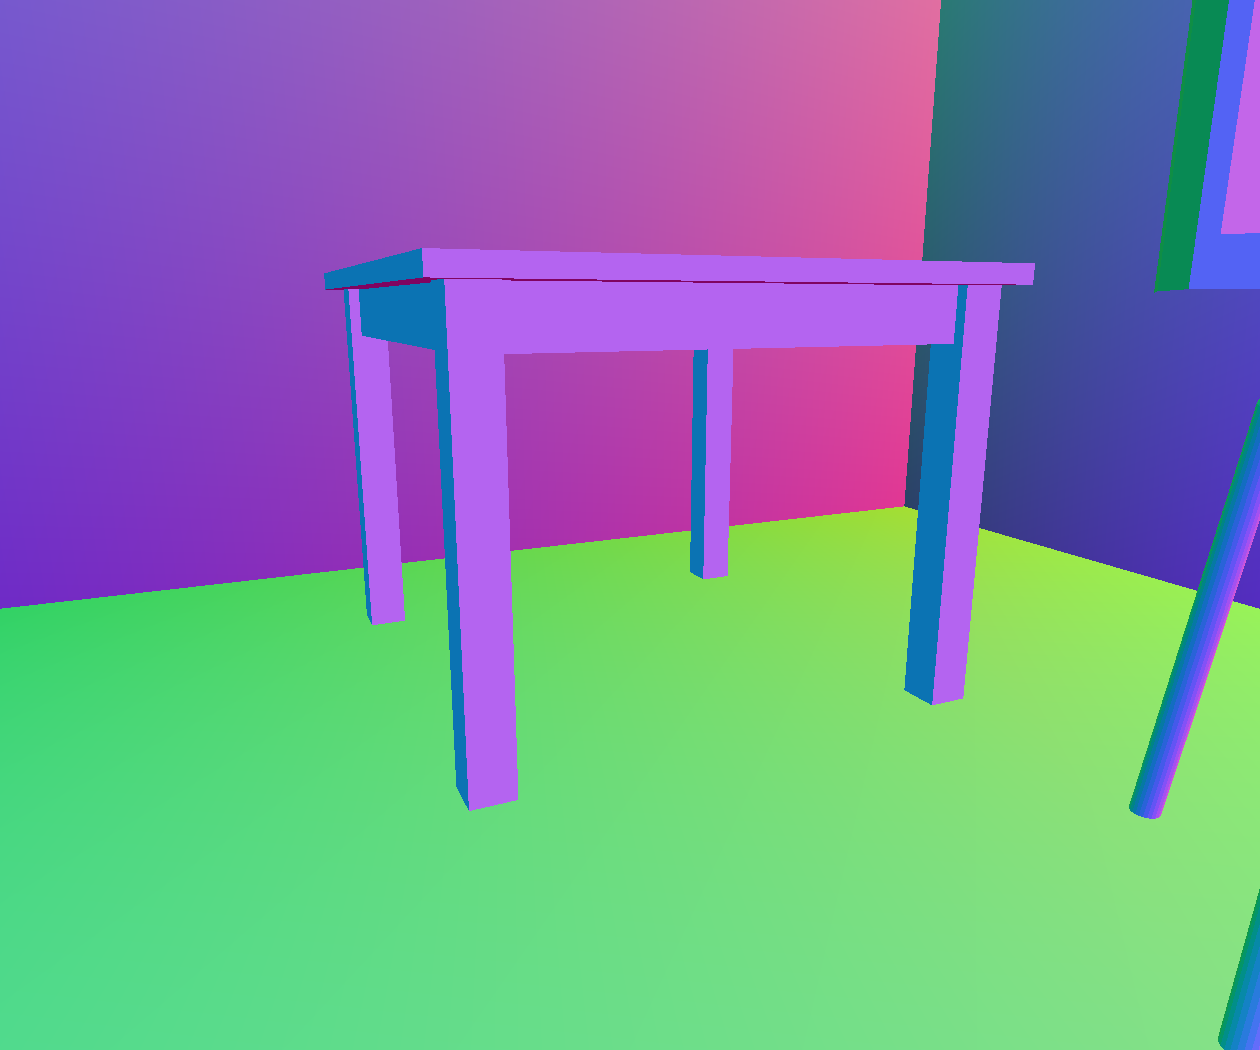
\includegraphics[width=.19\linewidth]{/Users/apple/OVGU/Thesis/code/3dReconstruction/report/images/implementation/gbuffers/4_normals}\\
    \vspace{0.1cm}

        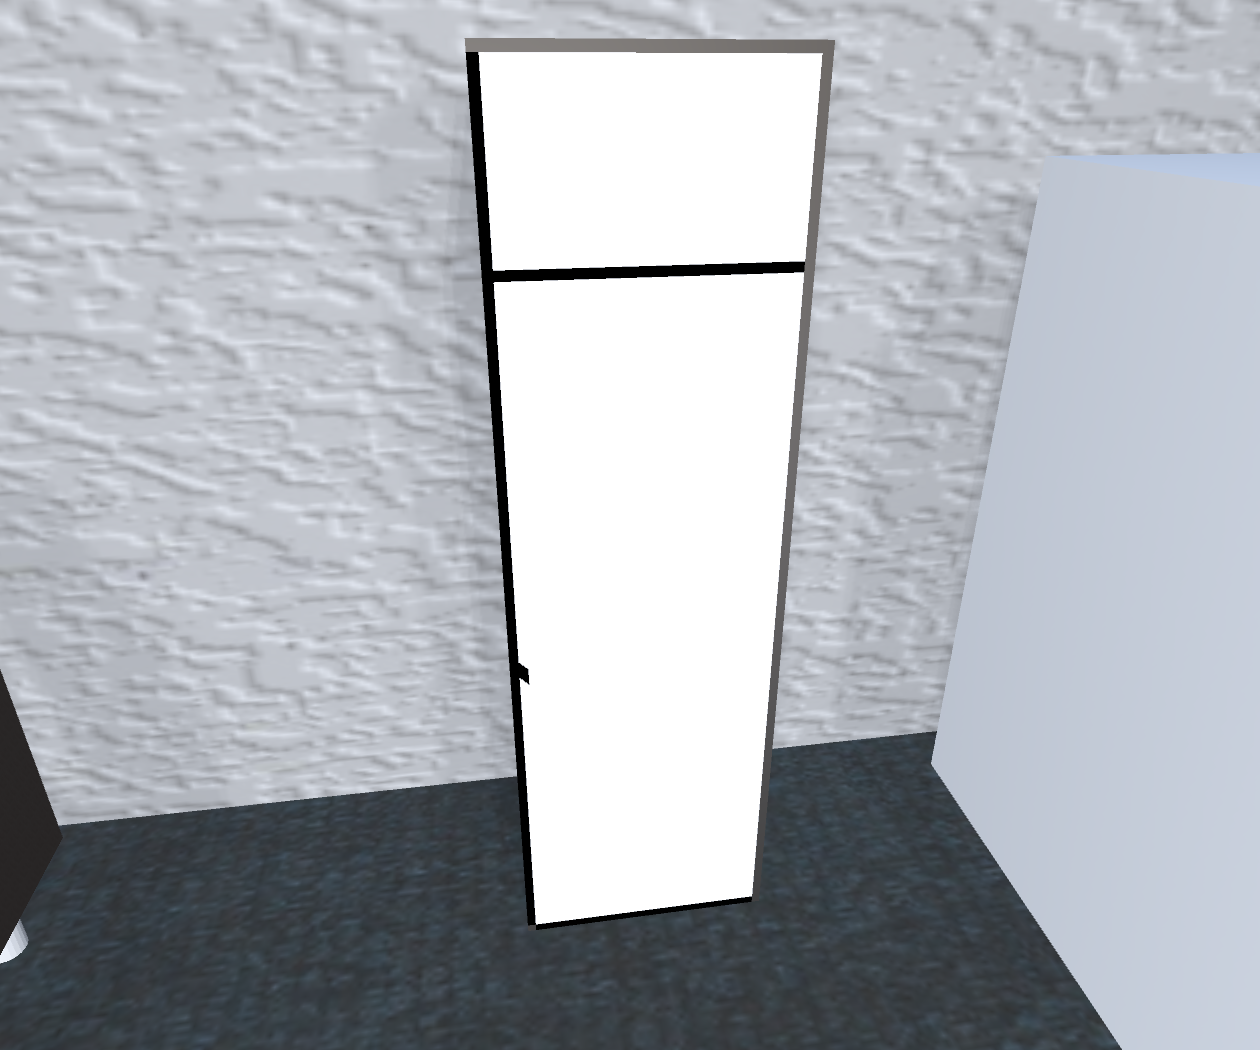
\includegraphics[width=.19\linewidth]{/Users/apple/OVGU/Thesis/code/3dReconstruction/report/images/implementation/gbuffers/5_img}
        
\includegraphics[width=.19\linewidth]{/Users/apple/OVGU/Thesis/code/3dReconstruction/report/images/implementation/gbuffers/5_depth}
        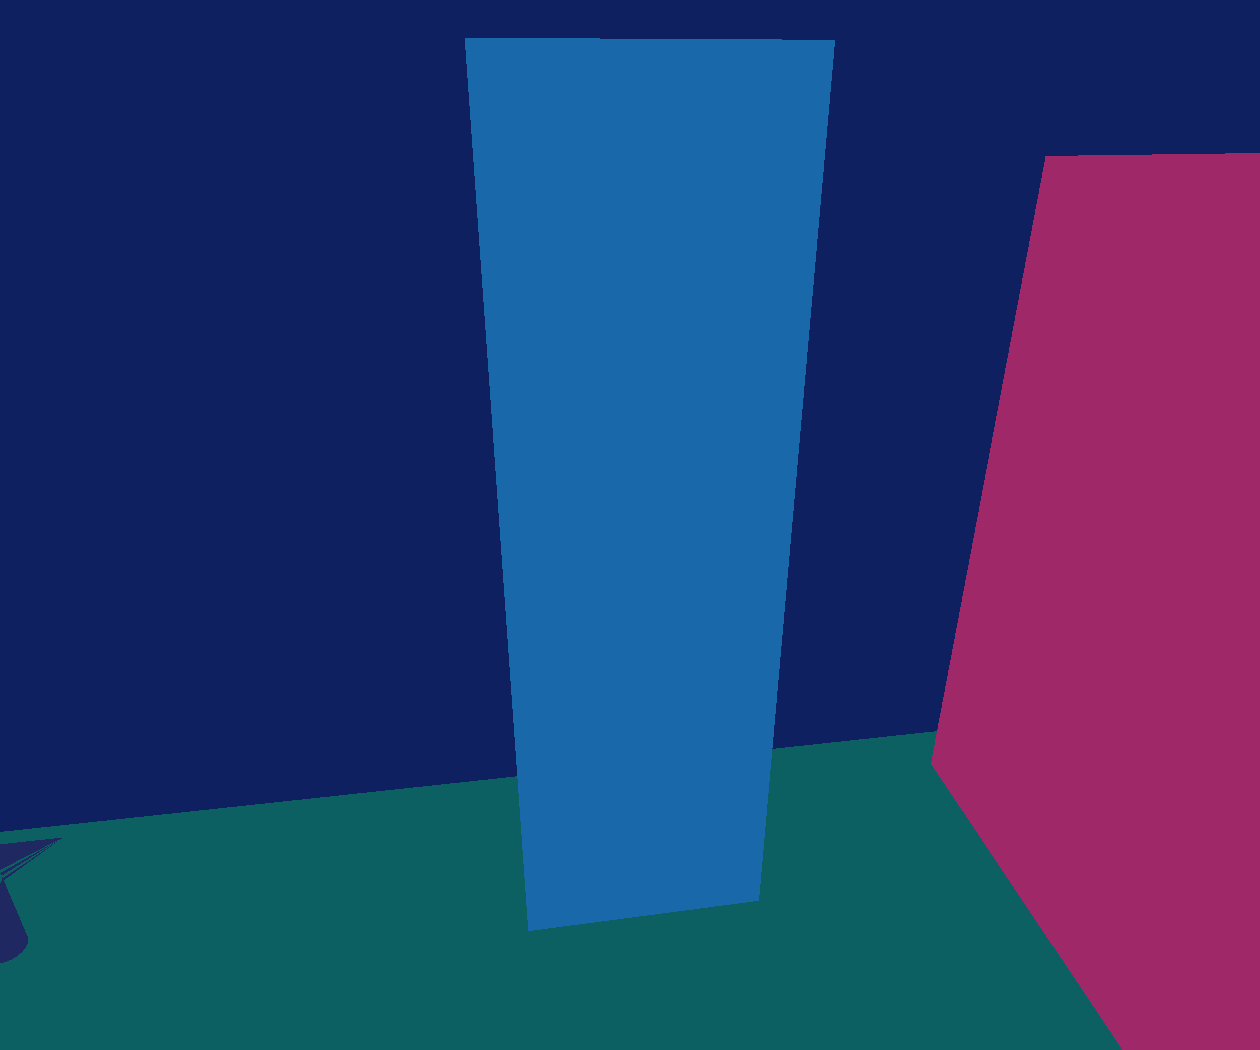
\includegraphics[width=.19\linewidth]{/Users/apple/OVGU/Thesis/code/3dReconstruction/report/images/implementation/gbuffers/5_id}
        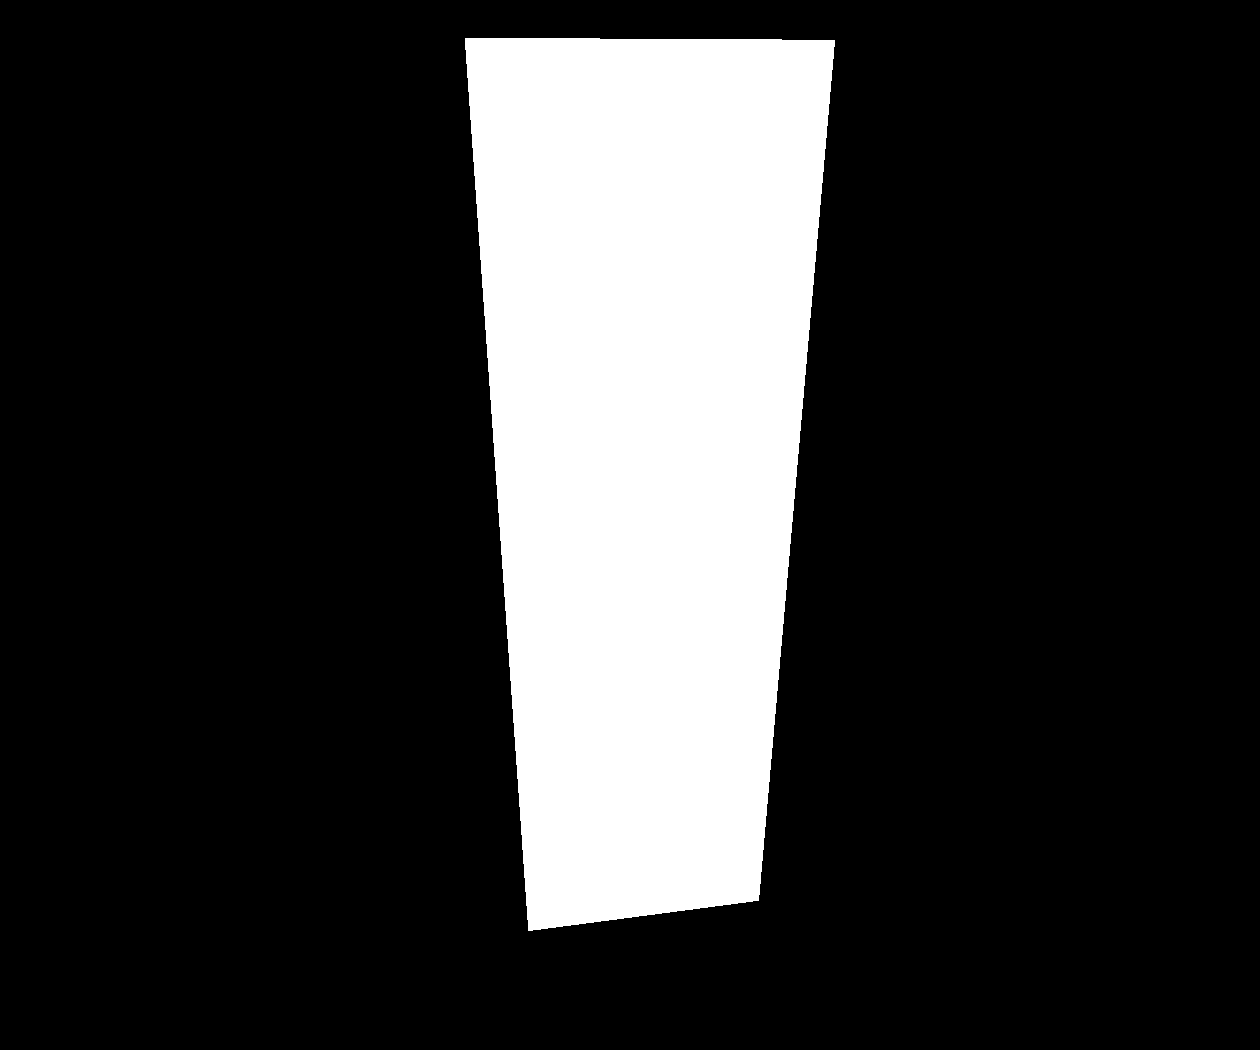
\includegraphics[width=.19\linewidth]{/Users/apple/OVGU/Thesis/code/3dReconstruction/report/images/implementation/gbuffers/5_layer}
        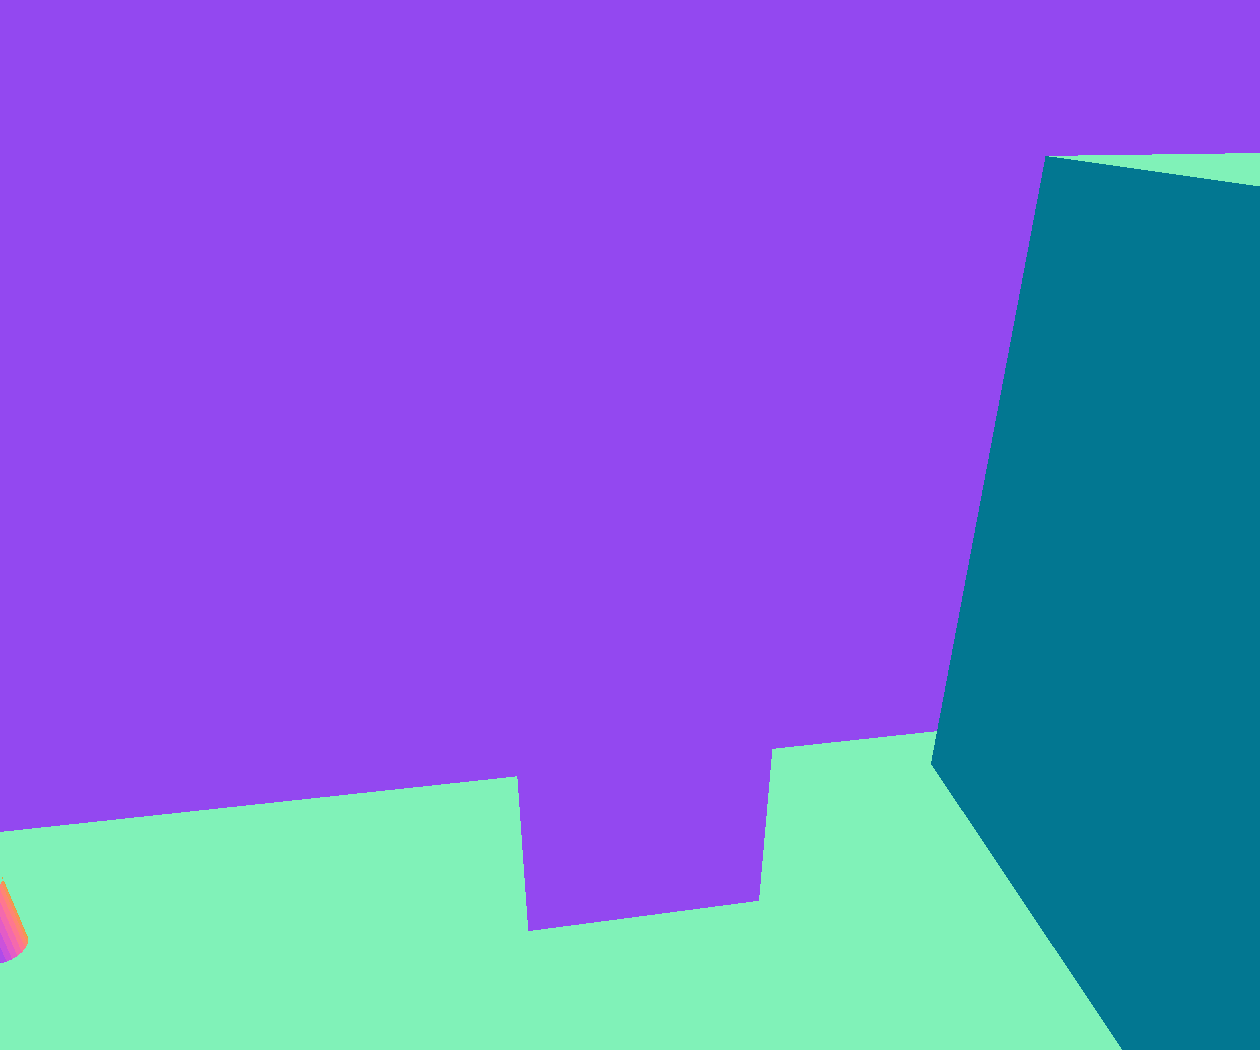
\includegraphics[width=.19\linewidth]{/Users/apple/OVGU/Thesis/code/3dReconstruction/report/images/implementation/gbuffers/5_normals}\\
    \vspace{0.1cm}

        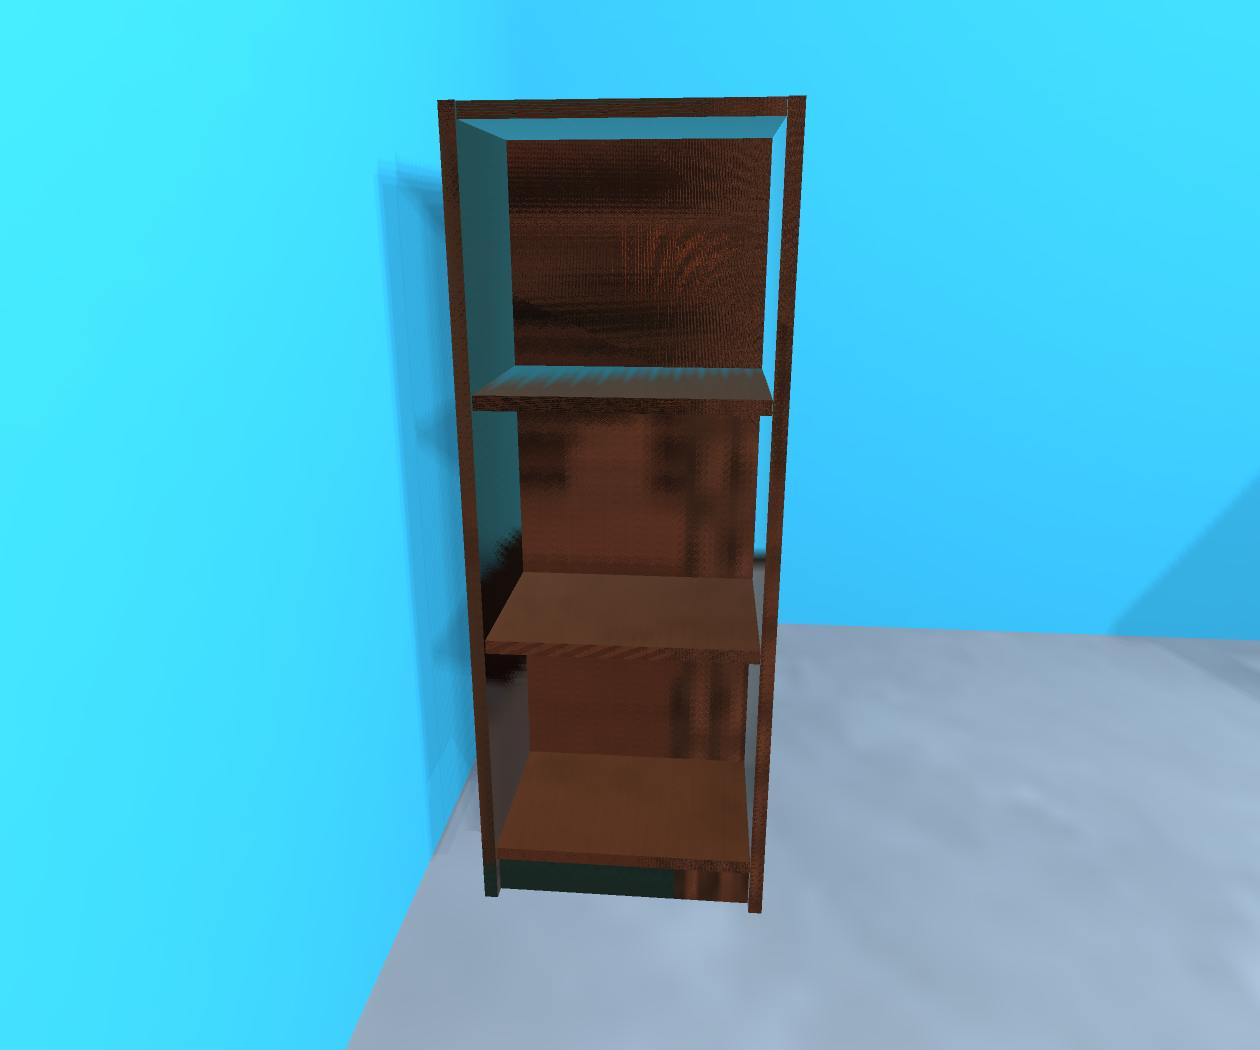
\includegraphics[width=.19\linewidth]{/Users/apple/OVGU/Thesis/code/3dReconstruction/report/images/implementation/gbuffers/6_img}
        
\includegraphics[width=.19\linewidth]{/Users/apple/OVGU/Thesis/code/3dReconstruction/report/images/implementation/gbuffers/6_depth}
        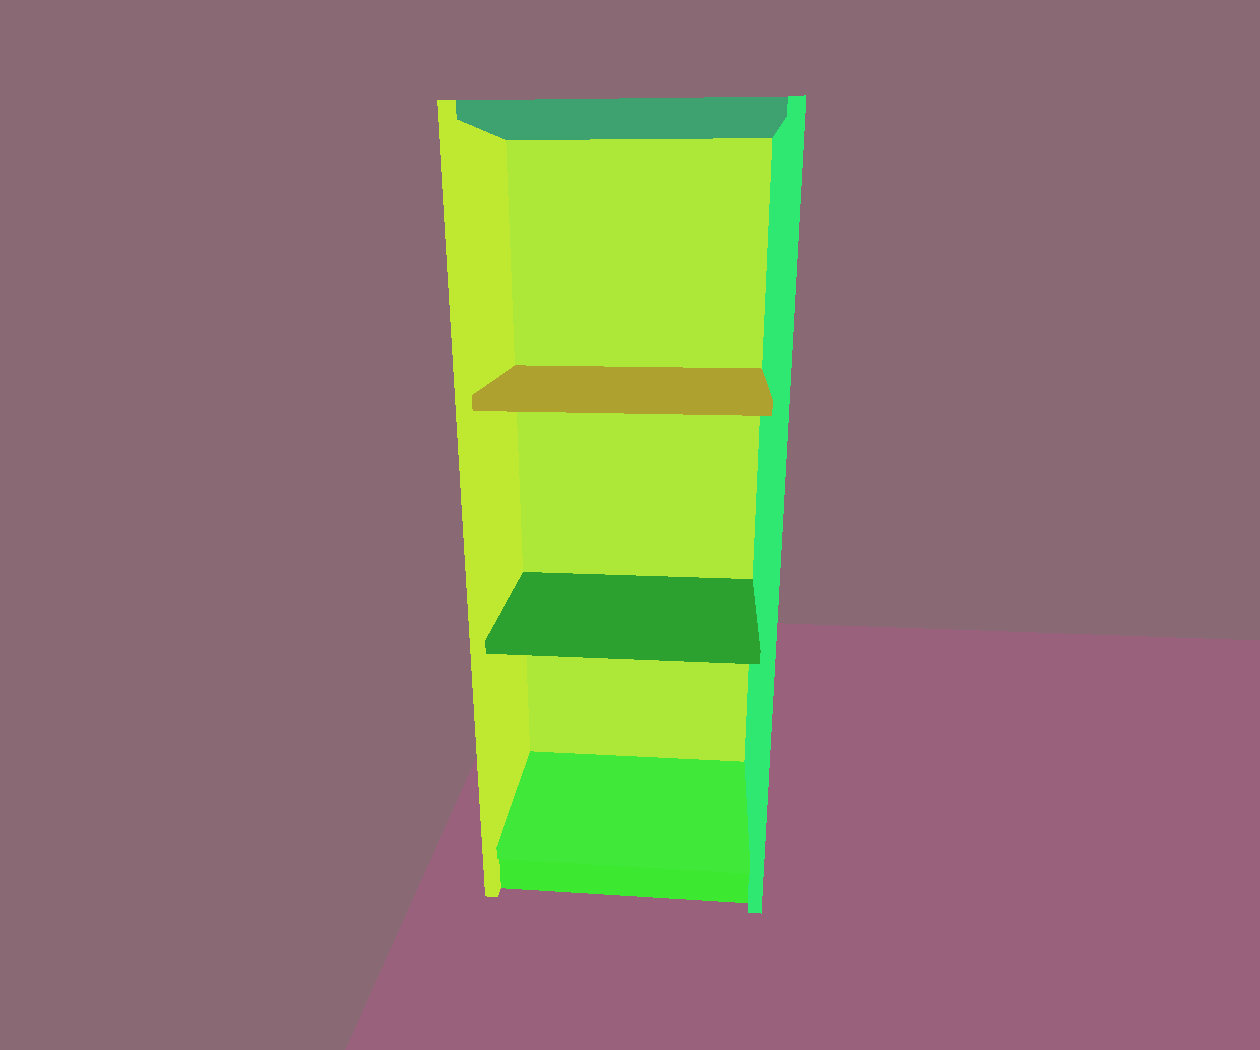
\includegraphics[width=.19\linewidth]{/Users/apple/OVGU/Thesis/code/3dReconstruction/report/images/implementation/gbuffers/6_id}
        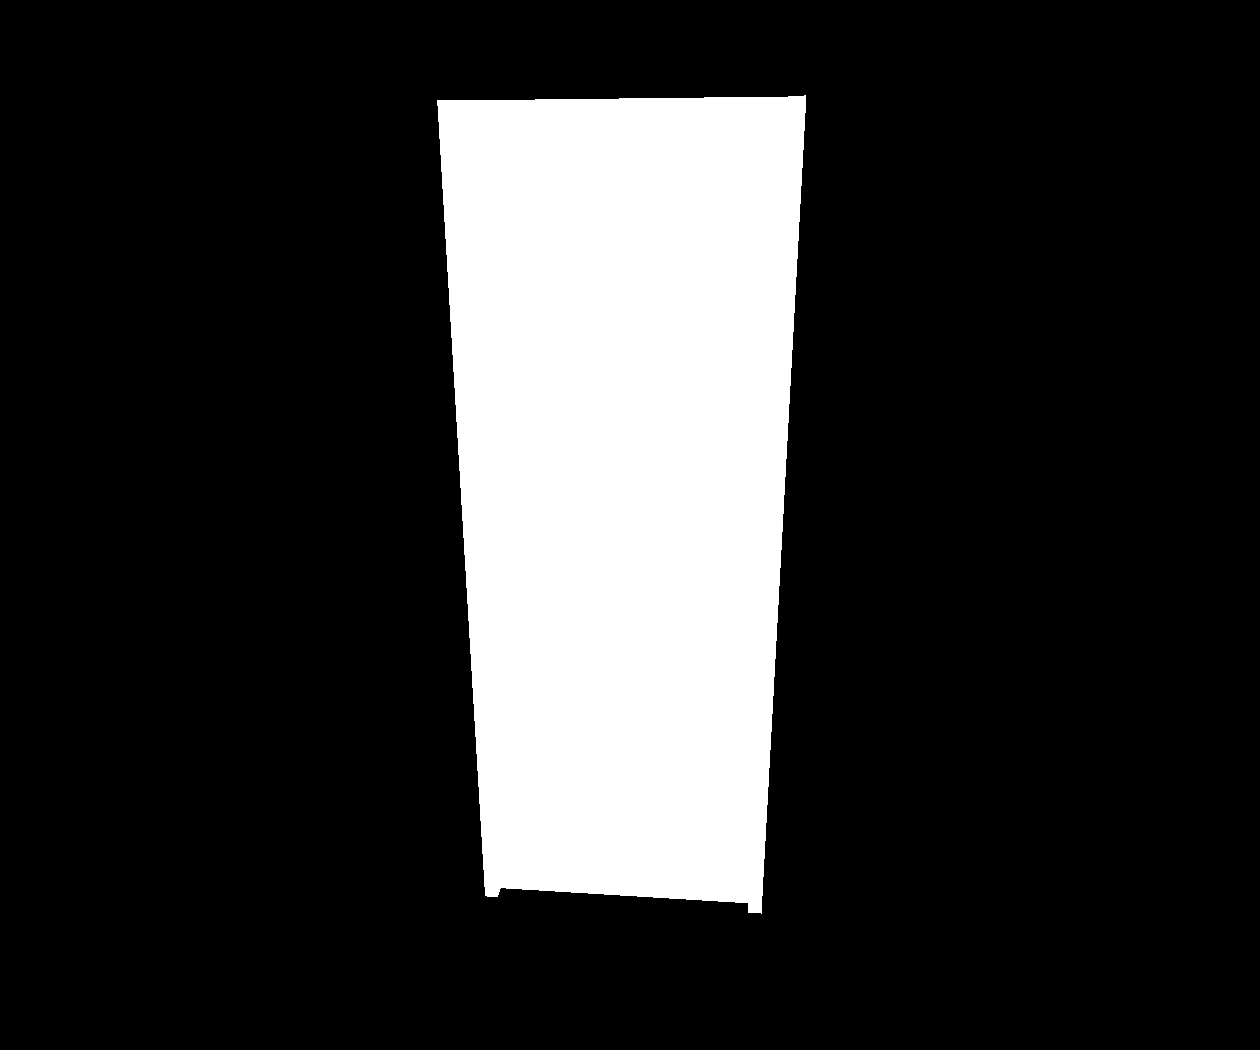
\includegraphics[width=.19\linewidth]{/Users/apple/OVGU/Thesis/code/3dReconstruction/report/images/implementation/gbuffers/6_layer}
        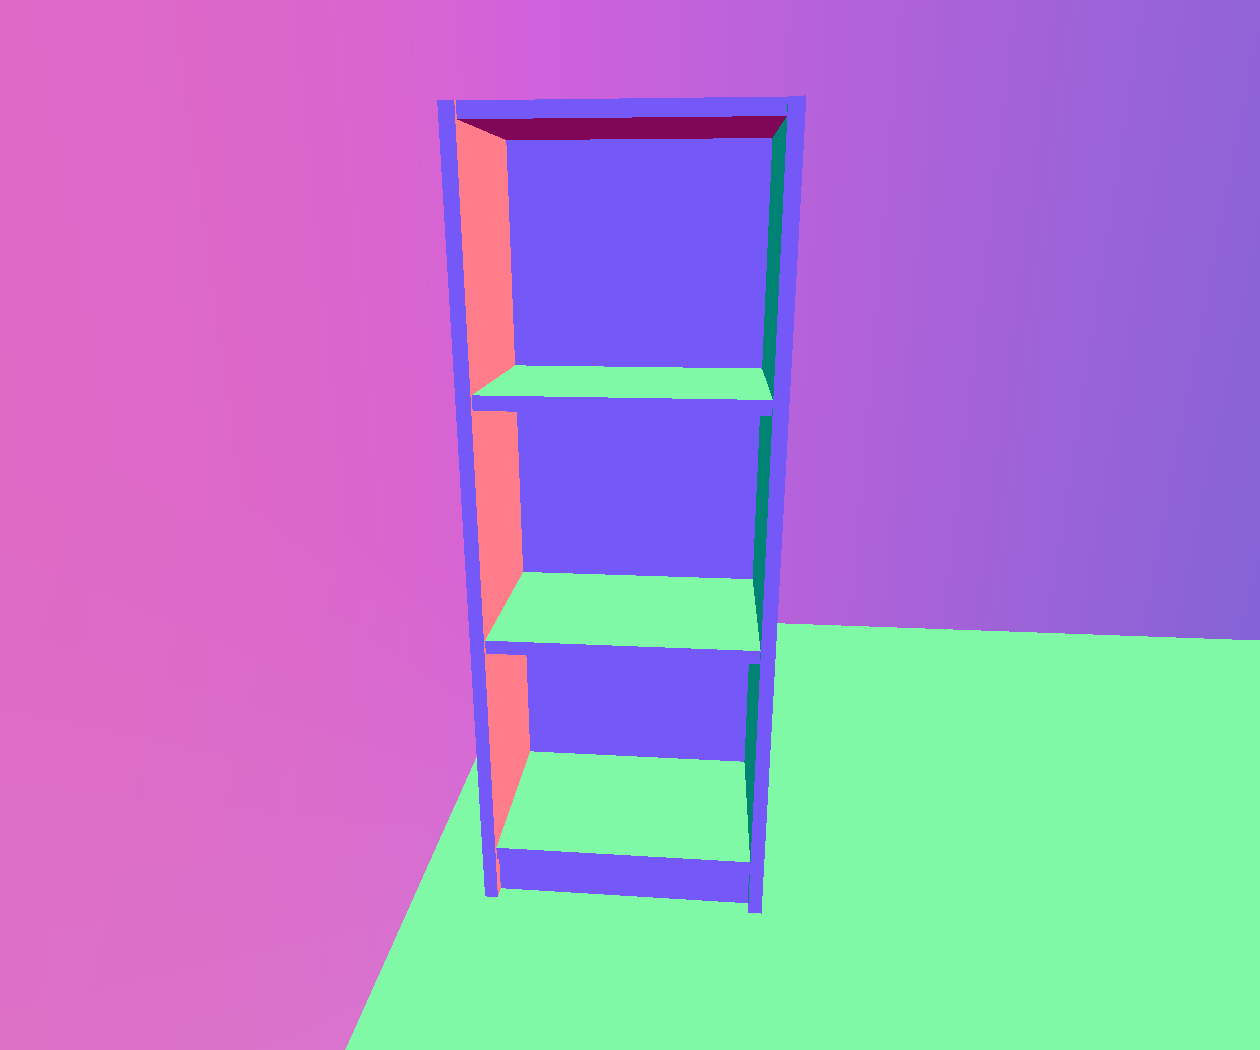
\includegraphics[width=.19\linewidth]{/Users/apple/OVGU/Thesis/code/3dReconstruction/report/images/implementation/gbuffers/6_normals}\\
    \caption{Samples for G-buffers collected from ImageSynthesis as part of the dataset. In the figure,
        (From left to right) RGB image, Depth map, Instance segmentation, Semantic Segmentation and Normal map}
    \label{fig:G-buffers-samples}
\end{figure}

\section{Demo for the application}\label{sec:demo}

The researchers are provided source code for the Unity-based application~\footnote{https://github.com/kartikprabhu20/3dScene}, which was used to create the synthetic datasets.
The application allows the users to provide paths for the 3D models, 3D rooms, textures, and output.
The user can also select the category of furniture for which images are to be generated and the quantity per category.
For the camera, the user can decide upon the height of the camera position, minimum and maximum distance from the target model, between which a viewpoint will be randomly chosen.
The modes are discussed in \autoref{subsec:modes-of-operations}, which can be select once all the data is configured.
For the manual mode, the user can randomize one or more parameters and take the snapshot as desired.
\autoref{fig:demo1} shows the configuration page for the demo application, and \autoref{fig:demo2} shows the application in action in manual mode.

\begin{figure}
    \centering
    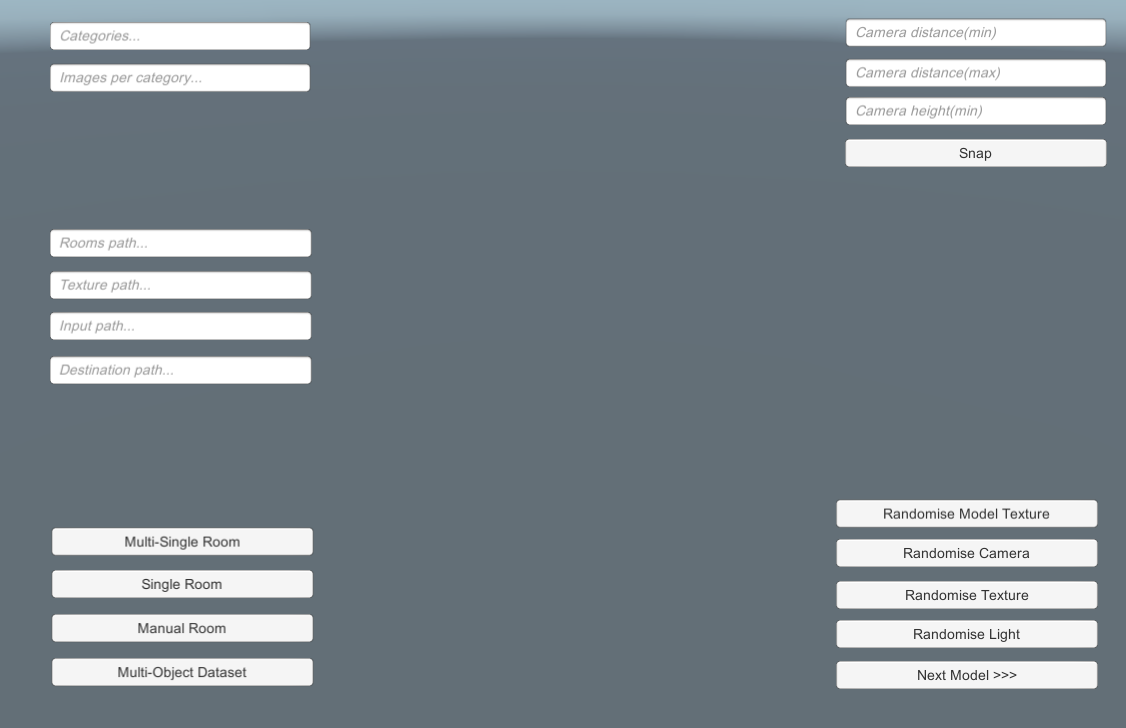
\includegraphics[width=\textwidth]{/Users/apple/OVGU/Thesis/code/3dReconstruction/report/images/implementation/demo/demo}
    \caption{A screenshot of the Unity based application developed for proof of concept to create synthetic dataset.}
    \label{fig:demo1}
\end{figure}

\begin{figure}
    \centering
    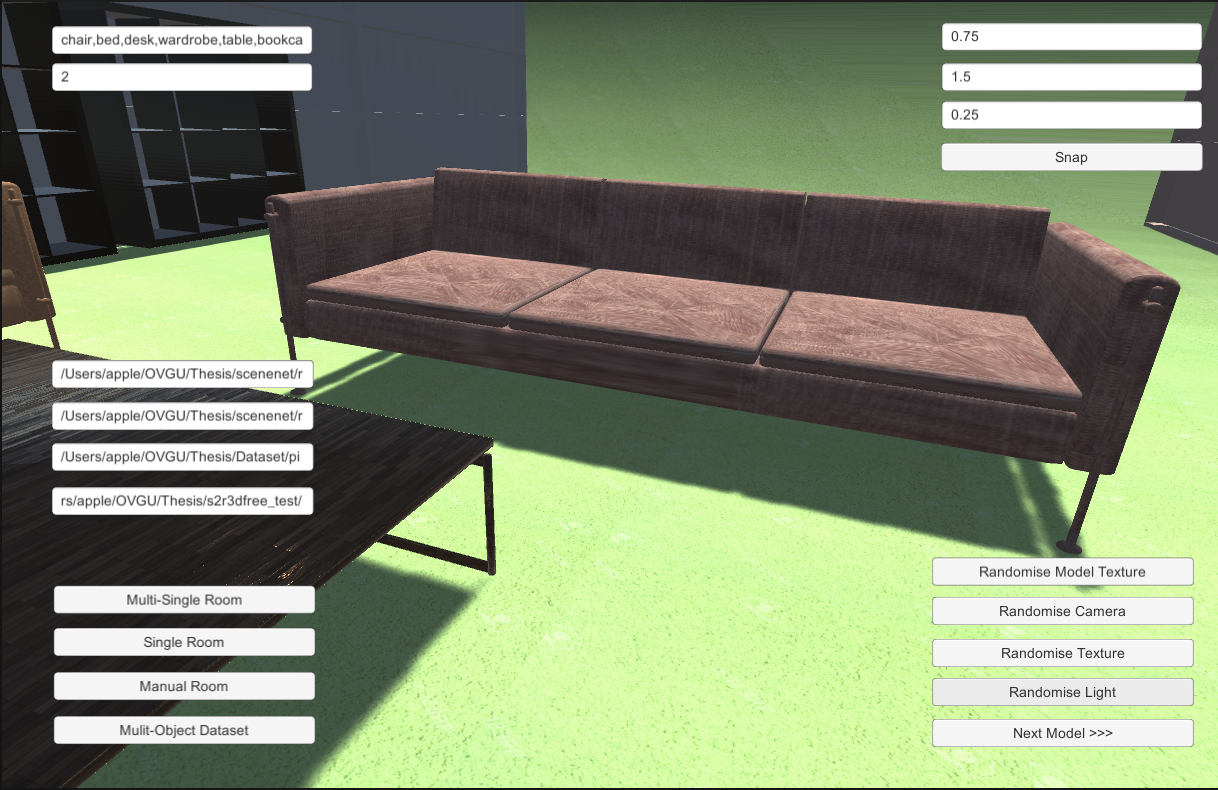
\includegraphics[width=\textwidth]{/Users/apple/OVGU/Thesis/code/3dReconstruction/report/images/implementation/demo/demo2}
    \caption{A screenshot of the Unity based application in action, the user is able to configure the pipeline using GUI and take snapshots either automatically or manually.}
    \label{fig:demo2}
\end{figure}

\section{3d-Reconstruction framework}\label{sec:3d-reconstruction-framework}

In this section, we discuss the pipeline used for the 3D reconstruction~\footnote{https://github.com/kartikprabhu20/3dReconstruction} tasks using Deep Learning.
The discussion will revolve around the implementation of models and the training parameters.
The code for the pipeline was written in Python 3.7.9.
The backbone of this pipeline is PyTorch 1.7.1~\cite{NEURIPS2019_9015}.

The key features of this pipeline are as follows:
\begin{enumerate}
    \item Allows users to configure the parameter using a config file which includes dataset paths, root paths, output path, parameters for 2D augmentations, etc.
    \item Allows users to select a train, validate, test with real data, an empty image test.
    \item Allows users to select the pipeline type(3d-reconstruction, cyclegan~\cite{CycleGAN2017}, autoencoder)
    \item Allows users to select the dataset(Pix3D, \gls(free), Mixed), with a further option to add new datasets.
    \item Allows users to collect graphs, images per epoch using Tensorboard~\footnote{https://www.tensorflow.org/}.
\end{enumerate}

\subsection{Preprocessing}\label{subsec:preprocessing}
As preprocessing for testing, images were resized to 224$\times$224 and then center cropped to 128$\times$128.
The images were then normalized using the parameters used for ImageNet~\cite{Deng2009ImageNetAL} Mean=[0.485, 0.456, 0.406] and STD=[0.229, 0.224, 0.225].
This was also done for training images followed by 2D-augmentations which included ColorJitter, RandomNoise, RandomFlip and, RandomPermuteRGB\@.
All the images were then transformed to a tensor to make them compatible with deep learning models.

\subsection{Modelling}\label{subsec:modelling}
For models, we used the architectures proposed in ~\cite{Xie_2019} and ~\cite{Xie_2020}.
The backbones of these two models are \gls{vgg} and \gls{resnet} respectively.
These models were obtained from PyTorch's model zoo, pre-trained on ImageNet.
The rest of the architecture was built using basic models using PyTorch.
The weights for the models were initialized using Glorot Initializer~\cite{Glorot2010UnderstandingTD}.

\subsection{Training}\label{subsec:training}

For training, the Deep learning models for the 3D reconstruction task the GPU used was NVIDIA DGX-1 with one node,
with 512 GB RAM, and 8x NVIDIA Tesla V100 GPU cards.
The hyperparameters were initially fine-tuned with a grid search approach and then trained on parameters on which the baselines were published.
The difference was not significant;
hence we decided to follow the hyperparameters used by the authors~\cite{Xie_2019}.
The only visible difference being the batch size, where we used the maximum possible value that would fit a 32GB memory of the used GPU\@.
The rest of the hyperparameters are as shown in \autoref{tab:hyperparameter}.
A more extensive hyperparameter optimization can be done in the future for better performance.
The model took up to 96 hours to train.


The users could decide when to write the training values in the Tensorboard in the config file.
The Tensorboard saves the loss values for not only each epoch but also the images of the 3d models for the configured epochs.
Tensorboard also has the capability to save 3D models, but we observed that the interface freezes and also occupies a larger storge.
Hence, we convert the 3D models into 2D images for visualization using Matplotlib.

\begin{table}[ht]
    \centering
    \begin{tabular}{|c |c |}
        \hline
        Hyperparameter & Value \\ [0.5ex]
        \hline\hline
        Optimizer & Adam(\beta_1 =.9, \beta_2=.999)\\
        \hline
        Weight Initializer & Glorot \\
        \hline
        Batch Size & 128  \\
        \hline
        Learning Rate & 0.001 \\
        \hline
        Epochs & 400\\
        \hline
        Loss & Binary Crossentropy\\
        \hline
    \end{tabular}
    \caption{Hyperparameters used for training 3d reconstruction models.}
    \label{tab:hyperparameter}
\end{table}

\subsection{Evaluation}\label{subsec:evaluation}

For evaluating the models, we use \gls{iou} as used in the original paper~\cite{Xie_2019}.
In the validation step, we compute the average ~\gls{iou} for each of the batches and store the best epoch value.
In the case where the value increases, we replace the best value and save the model state as the best model.
No thresholding is done during the validation step to apply binary cross-entropy.

As illustrated by~\cite{Tatarchenko2019}, mean \gls{iou} as a standalone measure might be misleading.
Since the voxel-based representation is volumetric, even with high \gls{iou}, we may see a bad reconstruction.
For this reason, we use the \gls{f1} as our second measure of evaluation, for which we dedicate \autoref{sec:study-with-f-score}.
\gls{f1} is the harmonic mean between precision and recall.
We further make sure the models are reconstructing the 3D models qualitatively by comparing the output and ground truth visually.

For the testing step, we use the test split from the real dataset(Pix3D).
In this step, we compute the average of each sample with different threshold values and select the best average value as our result.
The threshold values used are 0.05, 0.075, .1, .2, .3, .4, .5, .6, .7.
The average \gls{iou} values for each of the categories are also noted for real data tests.





